\documentclass[aspectratio=169,10pt]{beamer}

\usepackage[utf8]{inputenc}
\usepackage[vietnamese]{babel}
\usepackage{graphicx}
\usepackage{booktabs}
\usepackage{tabularx}
\usepackage{tikz}
\usepackage{amssymb}
\usepackage{pifont}
\usepackage{hyperref}

\usetheme{Madrid}
\usecolortheme{whale}

\definecolor{primary}{RGB}{30, 58, 138}
\definecolor{secondary}{RGB}{15, 118, 110}
\definecolor{accent}{RGB}{245, 158, 11}
\definecolor{darkslate}{RGB}{15, 23, 42}

\setbeamercolor{palette primary}{bg=primary,fg=white}
\setbeamercolor{palette secondary}{bg=secondary,fg=white}
\setbeamercolor{palette tertiary}{bg=darkslate,fg=white}
\setbeamercolor{structure}{fg=primary}
\setbeamercolor{titlelike}{parent=palette primary}
\setbeamercolor{block title}{bg=primary!15,fg=primary}
\setbeamercolor{block body}{bg=primary!5,fg=darkslate}

\setbeamertemplate{navigation symbols}{}
\setbeamertemplate{footline}{
  \leavevmode%
  \hbox{%
  \begin{beamercolorbox}[wd=.333333\paperwidth,ht=2.25ex,dp=1ex,left]{author in head/foot}%
    \usebeamerfont{author in head/foot}\hspace*{2ex}CryptoBot Architecture
  \end{beamercolorbox}%
  \begin{beamercolorbox}[wd=.333333\paperwidth,ht=2.25ex,dp=1ex,center]{title in head/foot}%
    \usebeamerfont{title in head/foot}HCMUS - KTPM
  \end{beamercolorbox}%
  \begin{beamercolorbox}[wd=.333333\paperwidth,ht=2.25ex,dp=1ex,right]{date in head/foot}%
    \usebeamerfont{date in head/foot}\insertframenumber{} / \inserttotalframenumber\hspace*{2ex}
  \end{beamercolorbox}}%
  \vskip0pt%
}

\title[CryptoBot Architecture]{\textbf{CRYPTO STRATEGY LAB (CryptoBot)}}
\subtitle{Báo Cáo Thiết Kế Kiến Trúc Phần Mềm (Software Architecture)}
\author[HCMUS - KTPM]{Nền tảng Nghiên cứu, Khám phá \& Đánh giá Chiến lược Tự động}
\institute[HCMUS]{Trường Đại học Khoa học Tự nhiên - ĐHQG-HCM \\ Bộ môn Kỹ thuật Phần mềm}
\date{\today}

\begin{document}

% Slide 1: Title
\begin{frame}
  \titlepage
\end{frame}

% Slide 2: Drivers
\begin{frame}{1. Bối cảnh \& 4 Nhóm Architectural Drivers Cốt lõi}
\begin{columns}[T]
\begin{column}{0.48\textwidth}
\begin{block}{\textbf{[Vấn đề \& Động lực]}}
\begin{itemize}
  \item \textbf{Realtime Market Ingestion:} Dữ liệu biến động mili-giây, cần stream liên tục \& tự phục hồi gap nến.
  \item \textbf{High Modifiability:} Bổ sung chiến lược mới (Handcraft/AI) không sửa core engine.
  \item \textbf{Massive Scalability:} Chạy hàng nghìn backtests song song không nghẽn UI.
  \item \textbf{Unstructured Intelligence:} Crawl tin tức đa nguồn, tự phục hồi khi HTML đổi cấu trúc.
\end{itemize}
\end{block}
\end{column}
\begin{column}{0.48\textwidth}
\begin{block}{\textbf{[Quyết định Kiến trúc Tương ứng]}}
\begin{itemize}
  \item \textbf{Driver 1 $\rightarrow$ Dual-Channel Ingestion:} Luồng Realtime WSS \& REST Backfill đồng nhất schema.
  \item \textbf{Driver 2 $\rightarrow$ Plugin \& AST Sandbox:} Chuẩn hóa contract \texttt{IStrategy}.
  \item \textbf{Driver 3 $\rightarrow$ Distributed Job Queue:} Phân tán tải qua Postgres Outbox \& Worker Leases.
  \item \textbf{Driver 4 $\rightarrow$ Multi-Agent Crawler:} Tự động nhận diện cấu trúc DOM \& chấm sentiment.
\end{itemize}
\end{block}
\end{column}
\end{columns}
\end{frame}

% Slide 3: Quality Attributes
\begin{frame}{2. Hệ Thống Quality Attributes (ASRs Taxonomy)}
\resizebox{\textwidth}{!}{%
\begin{tabular}{lp{5.2cm}p{6.8cm}}
\toprule
\textbf{Thuộc tính (QA)} & \textbf{Trọng tâm Thiết kế} & \textbf{Kỹ thuật / Tactic Kiến trúc áp dụng} \\
\midrule
\textbf{Modifiability} & Thêm Strategy, Search, Data Provider không sửa Core & Plugin Architecture, Open-Closed Principle, Dynamic Registry \\
\textbf{Scalability} & Xử lý đồng thời $>100,000$ backtests \& stream nến realtime & Scale-out Python Worker pool, Postgres Leased Job Queue, In-memory Broadcaster \\
\textbf{Realtime / Perf} & Độ trễ cập nhật nến $<200$ms, Backtest throughput cao & Go Edge Gateway, WebSocket Streaming, Deterministic Replay Engine \\
\textbf{Reliability} & Lỗi crawl/search không làm sập API; reconnect sàn & Failure Isolation, Transactional Outbox, Lease Takeover, Idempotency \\
\textbf{Observability} & Theo dõi Worker, tiến độ Search Loop \& nến realtime & Structured Logging, State Machine tracking, Loop Run Metrics \\
\textbf{Reproducibility} & Kết quả Backtest \& Leaderboard bất biến & Immutable Market Dataset snapshots, SHA-256 Run Hash, Seed Lock \\
\bottomrule
\end{tabular}}
\end{frame}

% Slide 4: ASR 1 & 2
\begin{frame}{3. Kịch Bản ASR Chi Tiết (Modifiability \& Scalability)}
\begin{columns}[T]
\begin{column}{0.48\textwidth}
\begin{block}{\textbf{[ASR-1: Modifiability (Thêm Strategy)]}}
\begin{itemize}
  \item \textbf{Source:} Quant Researcher / AI Agent.
  \item \textbf{Stimulus:} Thêm class chiến lược mới (\texttt{MACDStrategy}).
  \item \textbf{Artifact:} Strategy Subsystem \& UI Registry.
  \item \textbf{Response:} Tự động nạp metadata lên UI, không cần compile lại Go Gateway.
  \item \textbf{Measure:} 1 file Python độc lập, 0 downtime.
\end{itemize}
\end{block}
\end{column}
\begin{column}{0.48\textwidth}
\begin{block}{\textbf{[ASR-2: Scalability (Tải Backtest lớn)]}}
\begin{itemize}
  \item \textbf{Source:} Người dùng kích hoạt Auto Search Loop.
  \item \textbf{Stimulus:} 10,000 công việc backtest vào hàng đợi.
  \item \textbf{Artifact:} Job Queue \& Python Worker Pool.
  \item \textbf{Response:} Phân phối qua Lease Heartbeat, worker tự scale-out.
  \item \textbf{Measure:} Tỷ lệ hoàn thành 100\%, CPU/RAM ổn định.
\end{itemize}
\end{block}
\end{column}
\end{columns}
\end{frame}

% Slide 5: ASR 3 & 4
\begin{frame}{4. Kịch Bản ASR Chi Tiết (Realtime \& Reliability)}
\begin{columns}[T]
\begin{column}{0.48\textwidth}
\begin{block}{\textbf{[ASR-3: Realtime \& Data Parity]}}
\begin{itemize}
  \item \textbf{Source:} Sàn Binance (WSS drop/reconnect).
  \item \textbf{Stimulus:} Mất kết nối mạng trong 30 giây.
  \item \textbf{Artifact:} Go Market Gateway \& Postgres Storage.
  \item \textbf{Response:} Tự reconnect, REST Backfill bù nến thiếu, deduplicate bằng Open Time.
  \item \textbf{Measure:} Biểu đồ liên tục, độ trễ bắt kịp $<2$s.
\end{itemize}
\end{block}
\end{column}
\begin{column}{0.48\textwidth}
\begin{block}{\textbf{[ASR-4: Fault Tolerance (Worker Crash)]}}
\begin{itemize}
  \item \textbf{Source:} Python Worker bị kill đột ngột (OOM).
  \item \textbf{Stimulus:} Job đang ở trạng thái RUNNING.
  \item \textbf{Artifact:} Experiment Job Queue \& Outbox Manager.
  \item \textbf{Response:} Quá hạn Lease Heartbeat (30s), Worker khác tự động Takeover.
  \item \textbf{Measure:} Stuck job = 0, kết quả nhất quán.
\end{itemize}
\end{block}
\end{column}
\end{columns}
\end{frame}

% Slide 6: Use Case Diagram
\begin{frame}{5. Tổng Quan Use Case Hệ Thống}
\begin{columns}[c]
\begin{column}{0.45\textwidth}
\begin{itemize}
  \item \textbf{Quant Trader:} Xem biểu đồ nến realtime, khám phá chiến lược, chạy backtest, xem leaderboard.
  \item \textbf{AI Agent:} Tự crawl tin tức, trích xuất dữ liệu, chạy Loop Discovery tìm chiến lược tối ưu.
  \item \textbf{System Worker:} Nạp nến định kỳ, xử lý hàng đợi backtest bất đồng bộ.
\end{itemize}
\end{column}
\begin{column}{0.53\textwidth}
\centering
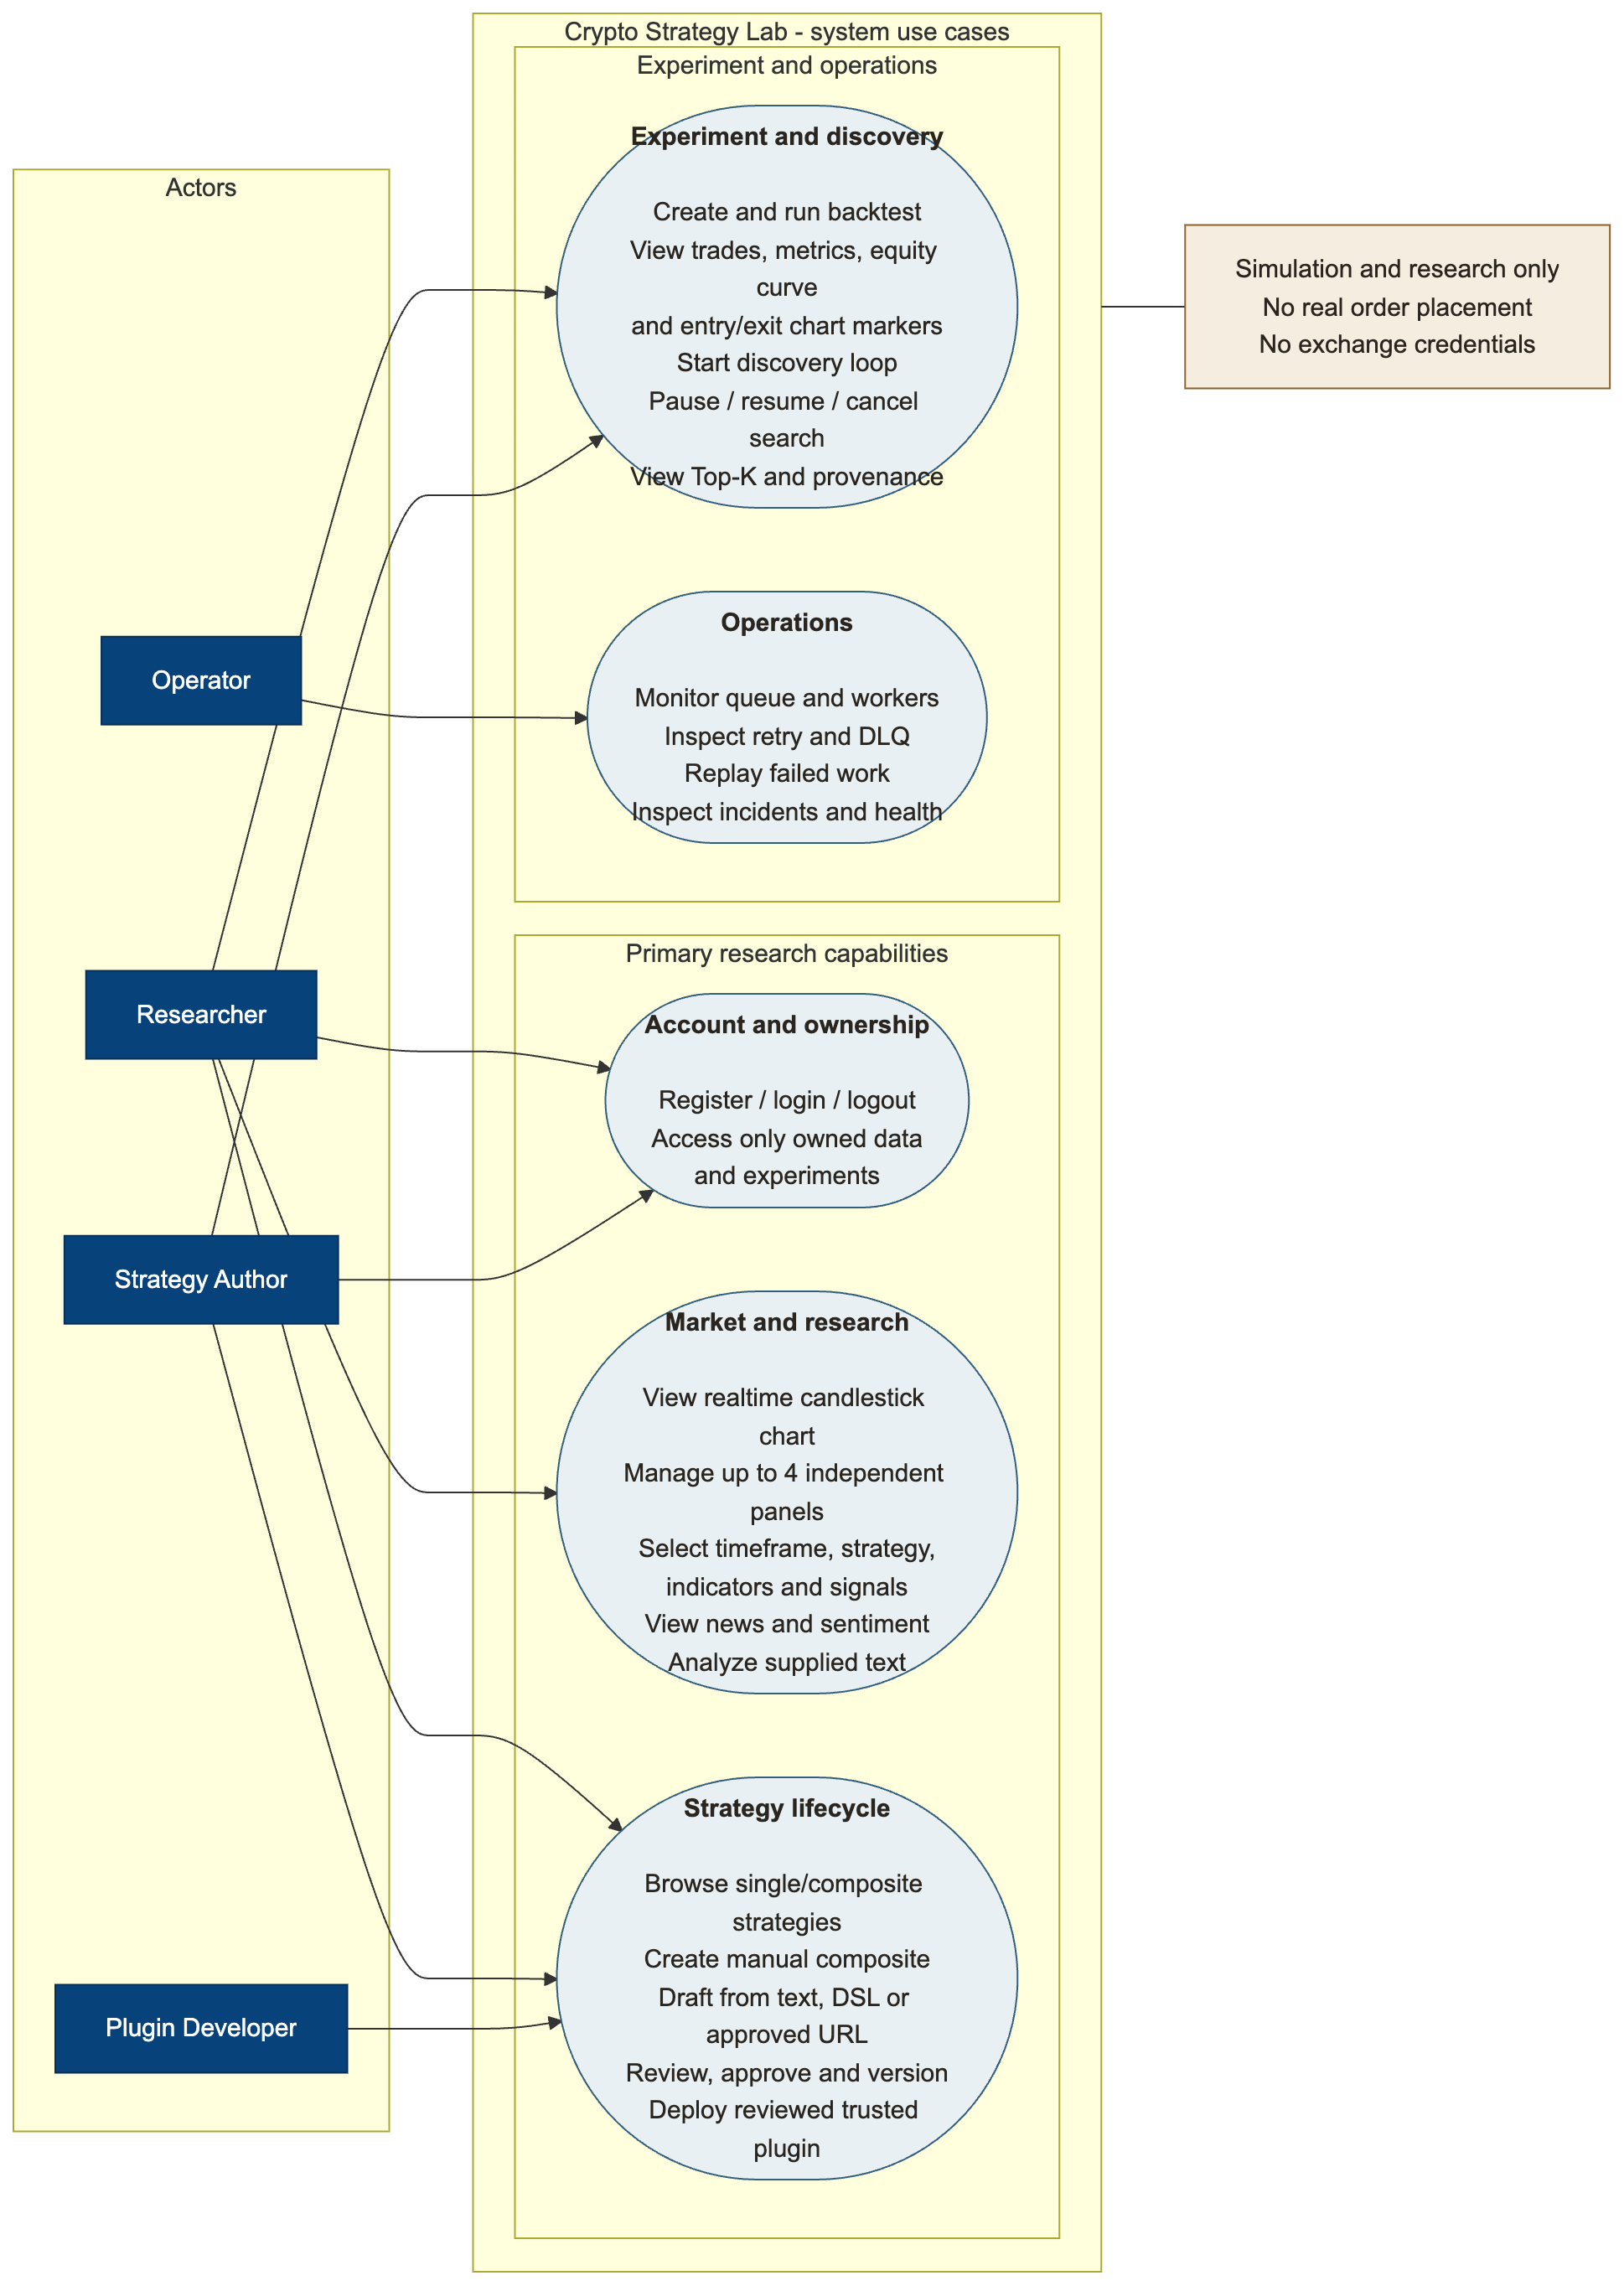
\includegraphics[width=\linewidth,height=0.75\textheight,keepaspectratio]{../blueprint/assets/diagrams-png/34-use-case-overview.png}
\end{column}
\end{columns}
\end{frame}

% Slide 7: C4 L1
\begin{frame}{6. C4 Model (Level 1) - System Context Diagram}
\begin{columns}[c]
\begin{column}{0.45\textwidth}
\begin{itemize}
  \item \textbf{CryptoBot Platform:} Hệ thống trung tâm phân tích thị trường, nghiên cứu chiến lược và chấm điểm.
  \item \textbf{External Systems:}
  \begin{itemize}
    \item \textbf{Binance Exchange:} REST \& WebSocket.
    \item \textbf{News / RSS Feeds:} Cung cấp tin thị trường.
    \item \textbf{LLM Providers (OpenAI/Groq):} Suy luận ngôn ngữ, sentiment \& self-repair code.
  \end{itemize}
\end{itemize}
\end{column}
\begin{column}{0.53\textwidth}
\centering
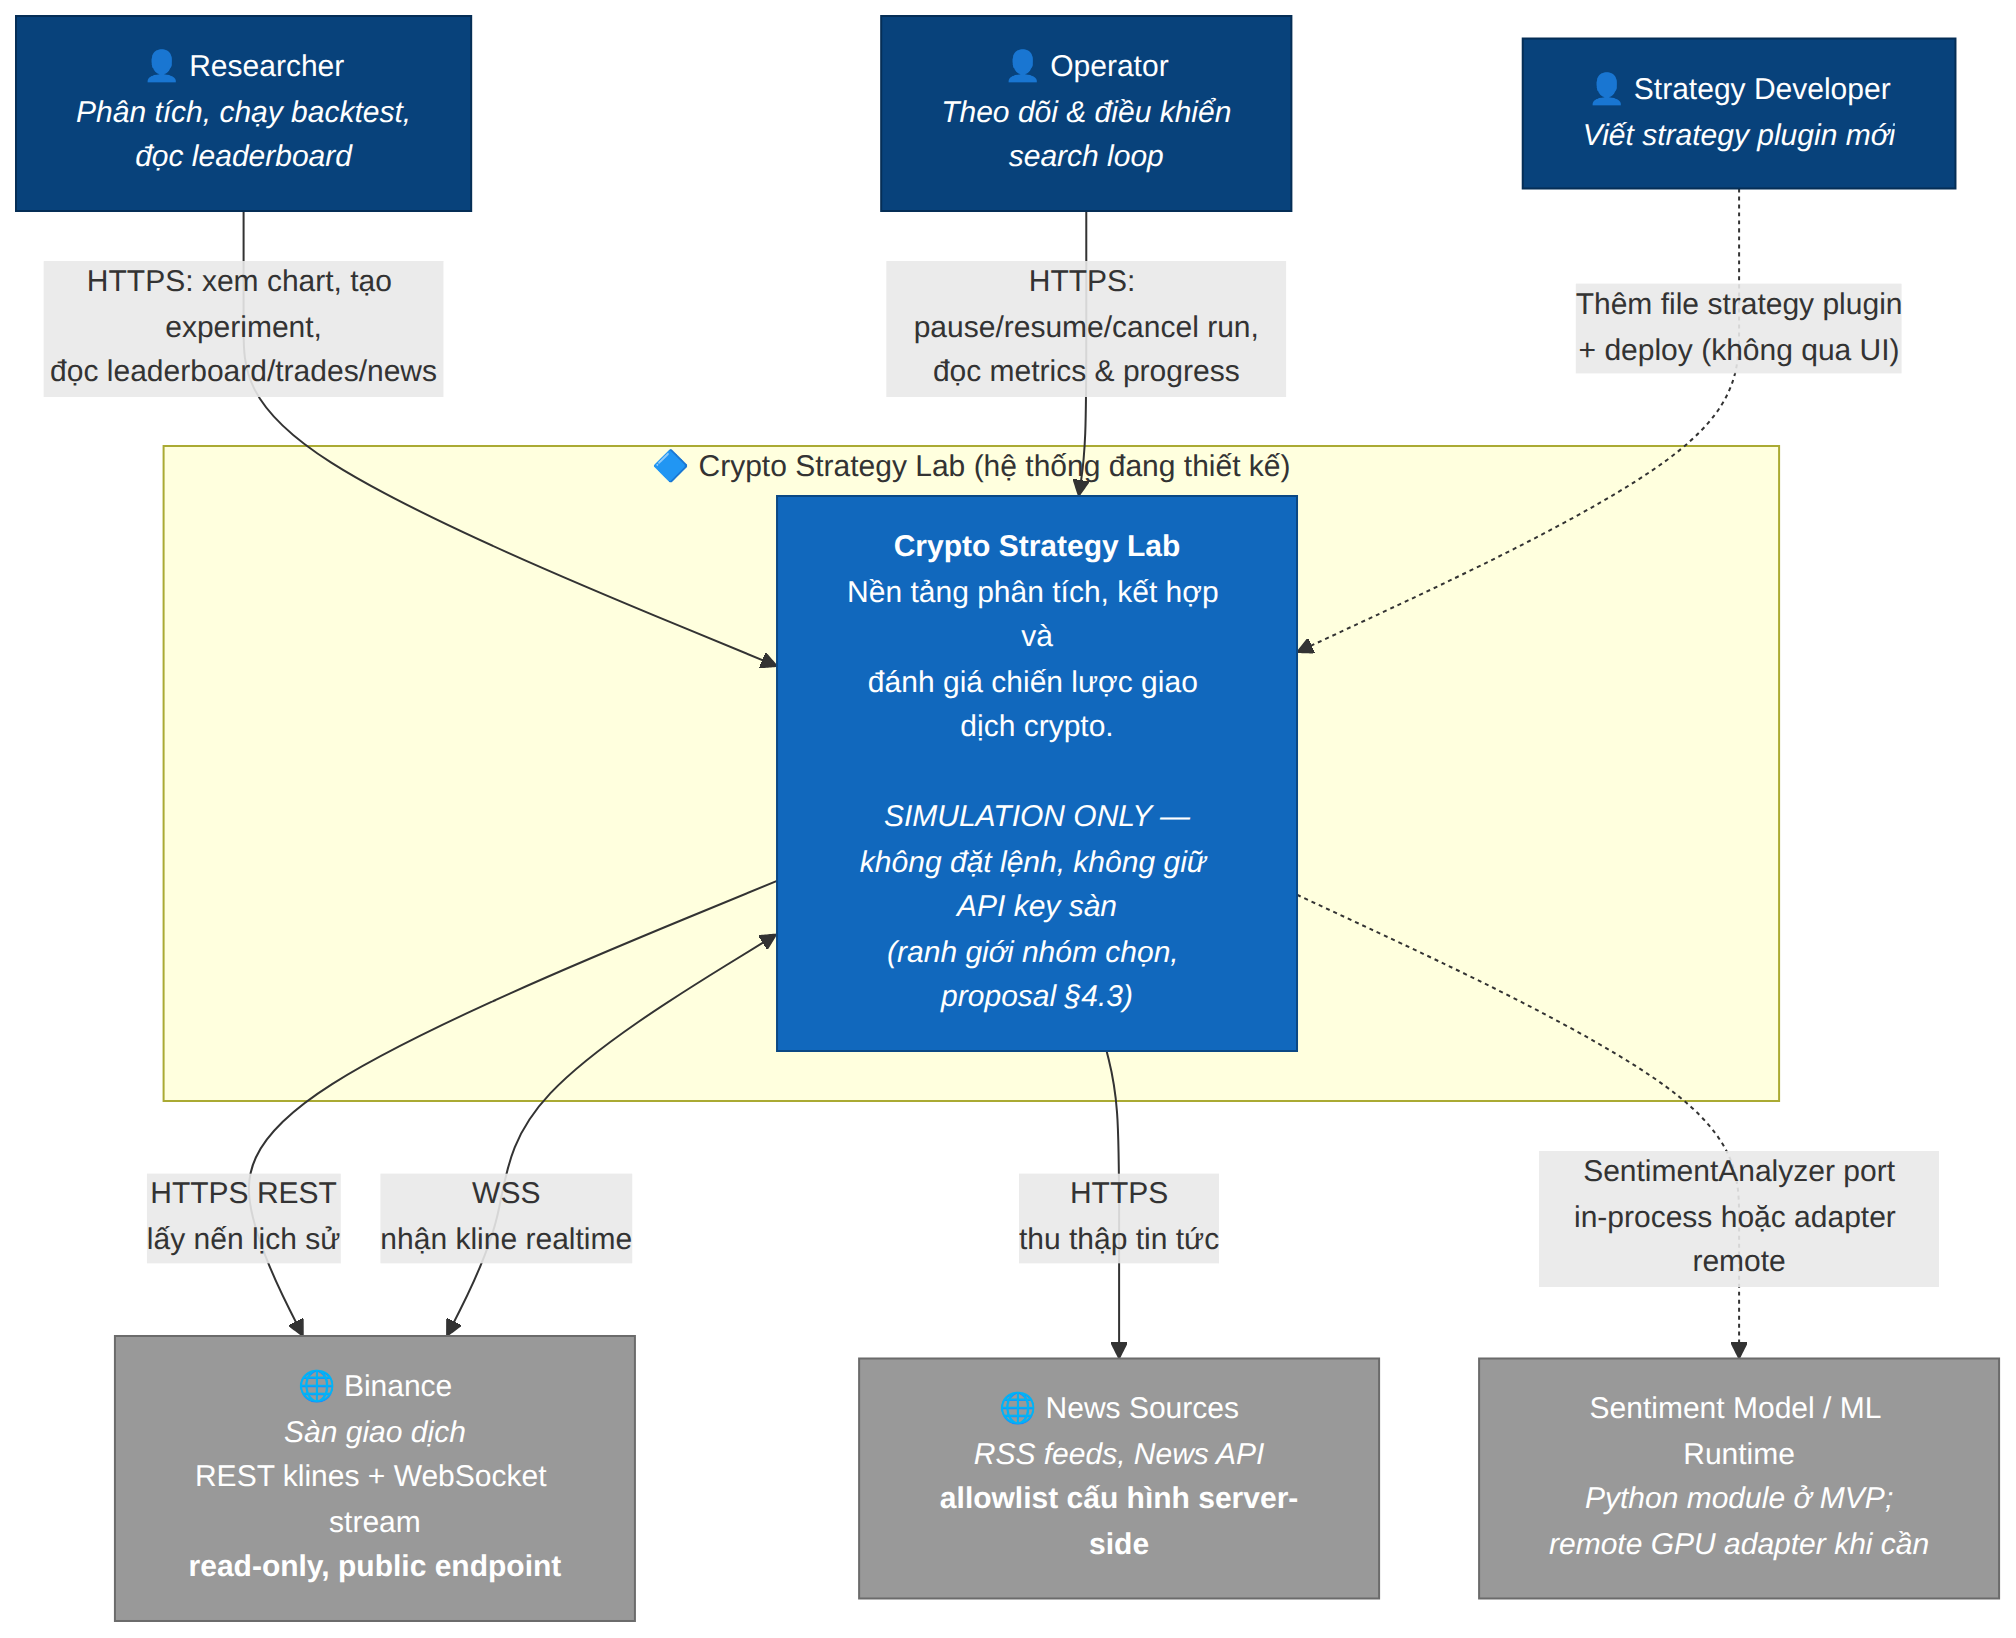
\includegraphics[width=\linewidth,height=0.75\textheight,keepaspectratio]{../blueprint/assets/diagrams-png/01-c4-l1-system-context.png}
\end{column}
\end{columns}
\end{frame}

% Slide 8: C4 L2
\begin{frame}{7. C4 Model (Level 2) - Container Diagram}
\begin{columns}[c]
\begin{column}{0.45\textwidth}
\begin{itemize}
  \item \textbf{Next.js Web App:} SPA tương tác, realtime chart, cấu hình chiến lược \& leaderboard.
  \item \textbf{Go Edge Gateway:} RBAC, CQRS routing, WebSocket streaming.
  \item \textbf{Python Research Engine:} Backtest worker, Loop discovery, Metric evaluation.
  \item \textbf{PostgreSQL Storage:} ACID Outbox, Candle store \& Job queue.
\end{itemize}
\end{column}
\begin{column}{0.53\textwidth}
\centering
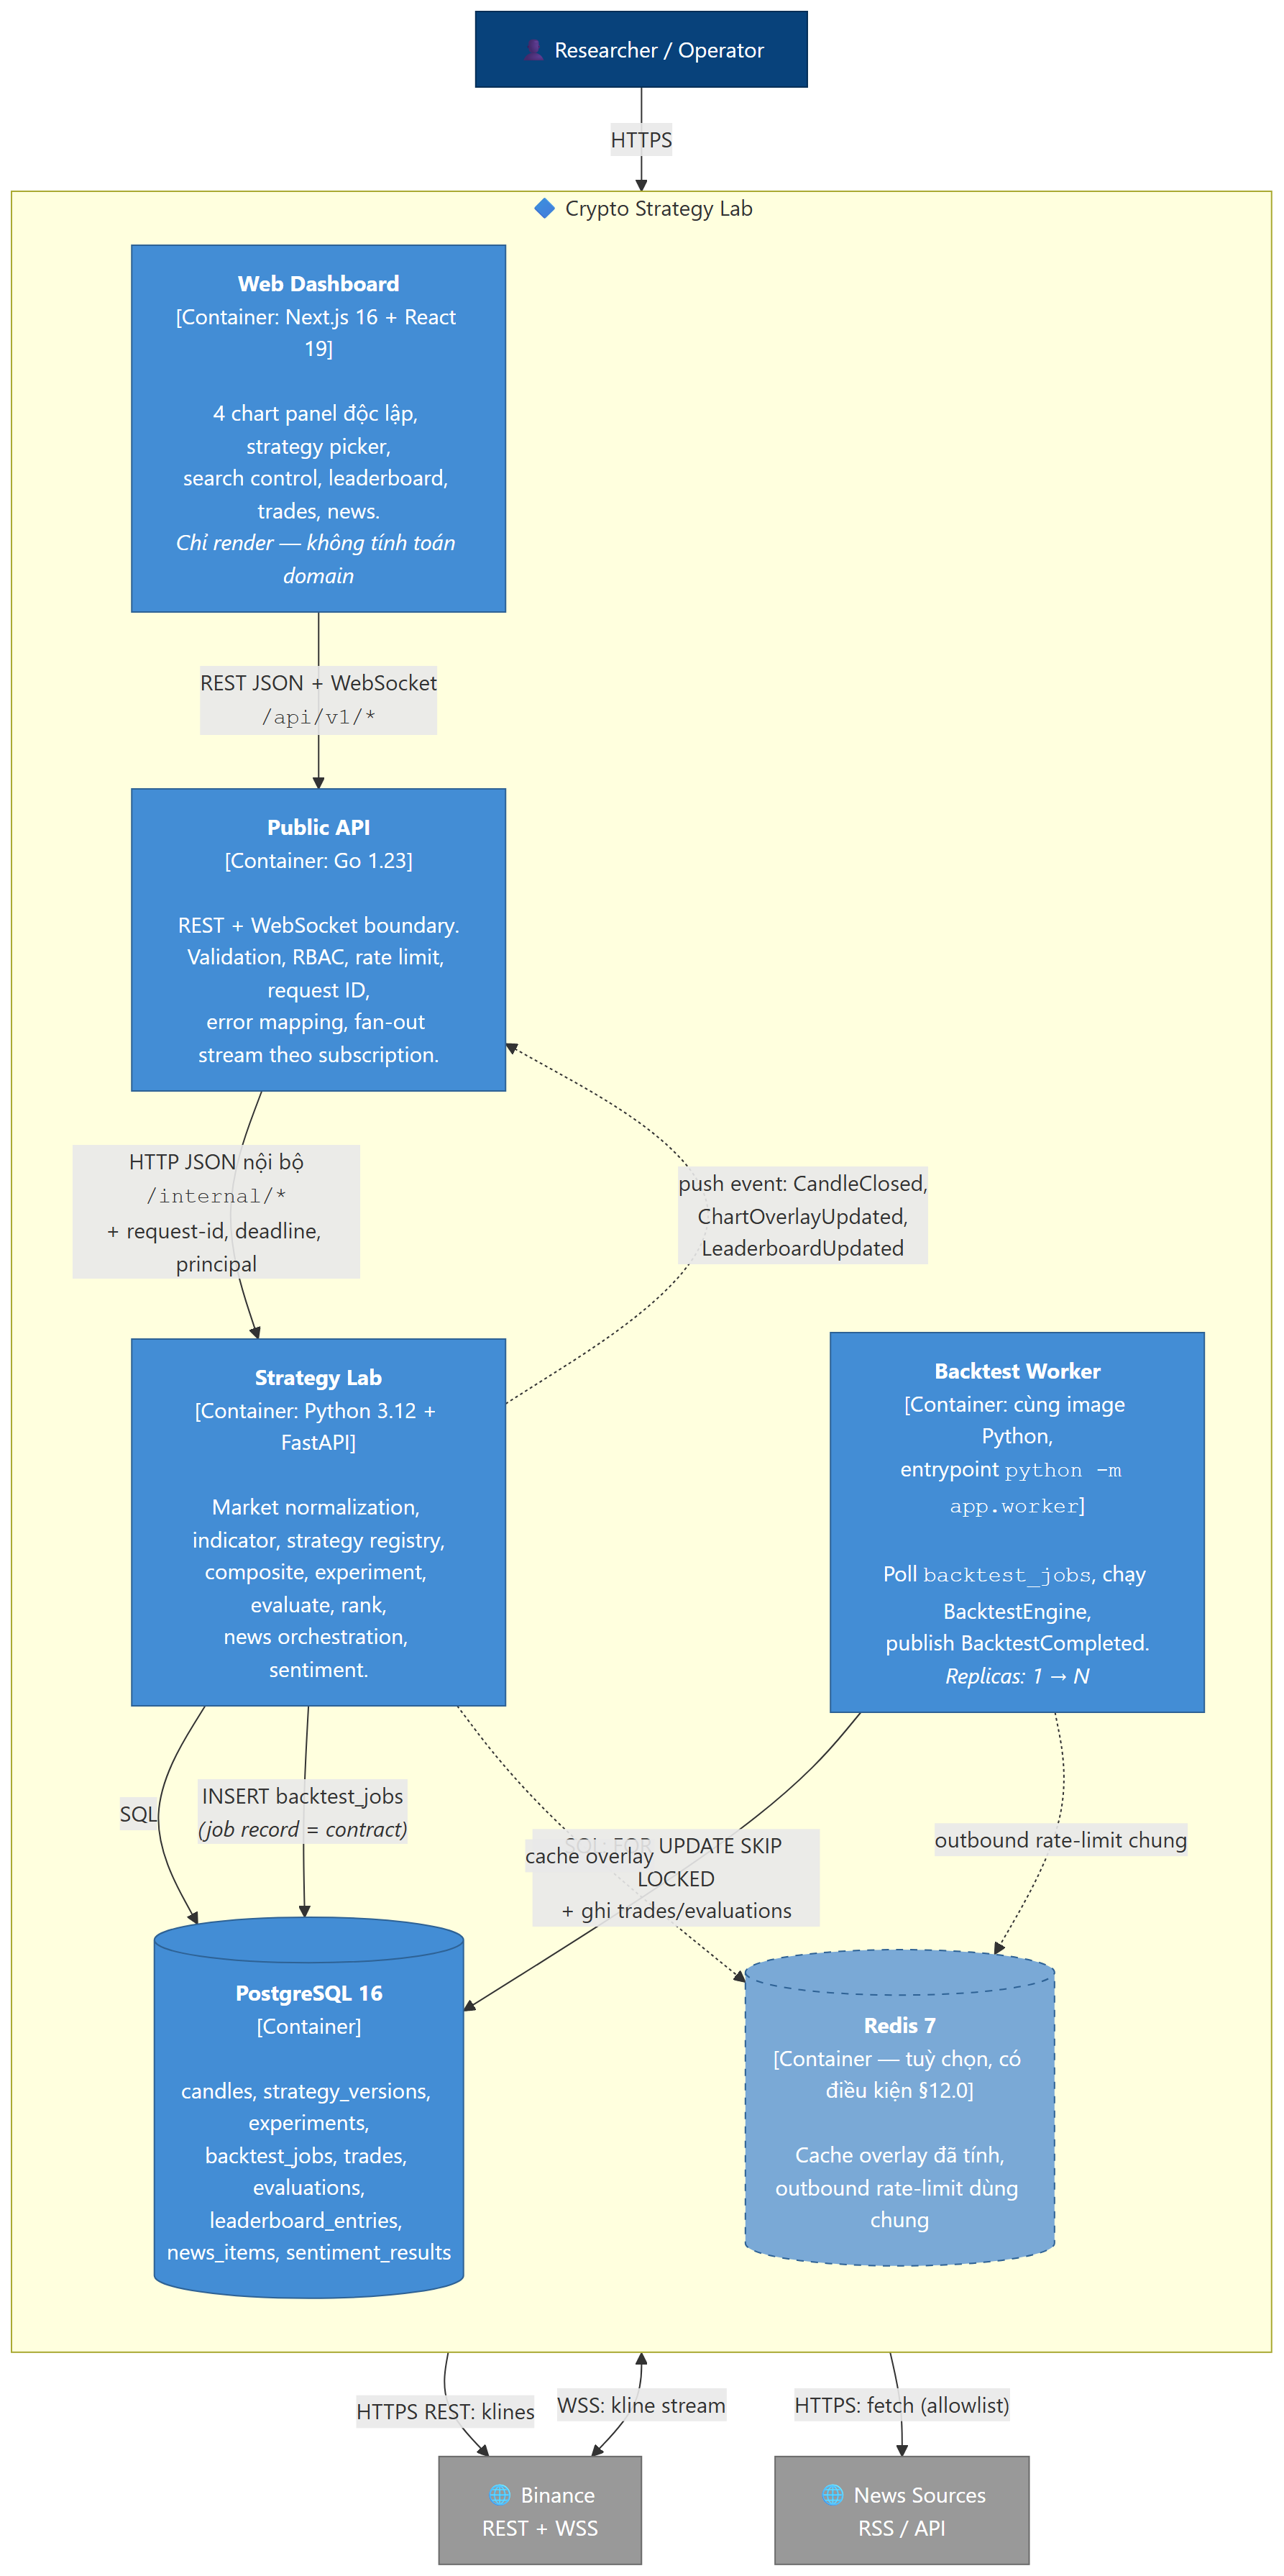
\includegraphics[width=\linewidth,height=0.75\textheight,keepaspectratio]{../blueprint/assets/diagrams-png/02-c4-l2-container.png}
\end{column}
\end{columns}
\end{frame}

% Slide 9: C4 L3 Python
\begin{frame}{8. C4 Model (Level 3) - Python Research Platform}
\begin{columns}[c]
\begin{column}{0.45\textwidth}
\begin{itemize}
  \item \textbf{Strategy Registry:} Quản lý lifecycle \& metadata plugin chiến lược.
  \item \textbf{Deterministic Backtest Engine:} Khớp lệnh chính xác (BBO, Slippage, Phí).
  \item \textbf{Search \& Loop Manager:} Genetic, Bayesian, Random search.
  \item \textbf{Worker Lease Manager:} Phân phối optimistic lock, tự phục hồi.
  \item \textbf{AST Sandbox:} Kiểm tra an toàn mã AI sinh.
\end{itemize}
\end{column}
\begin{column}{0.53\textwidth}
\centering
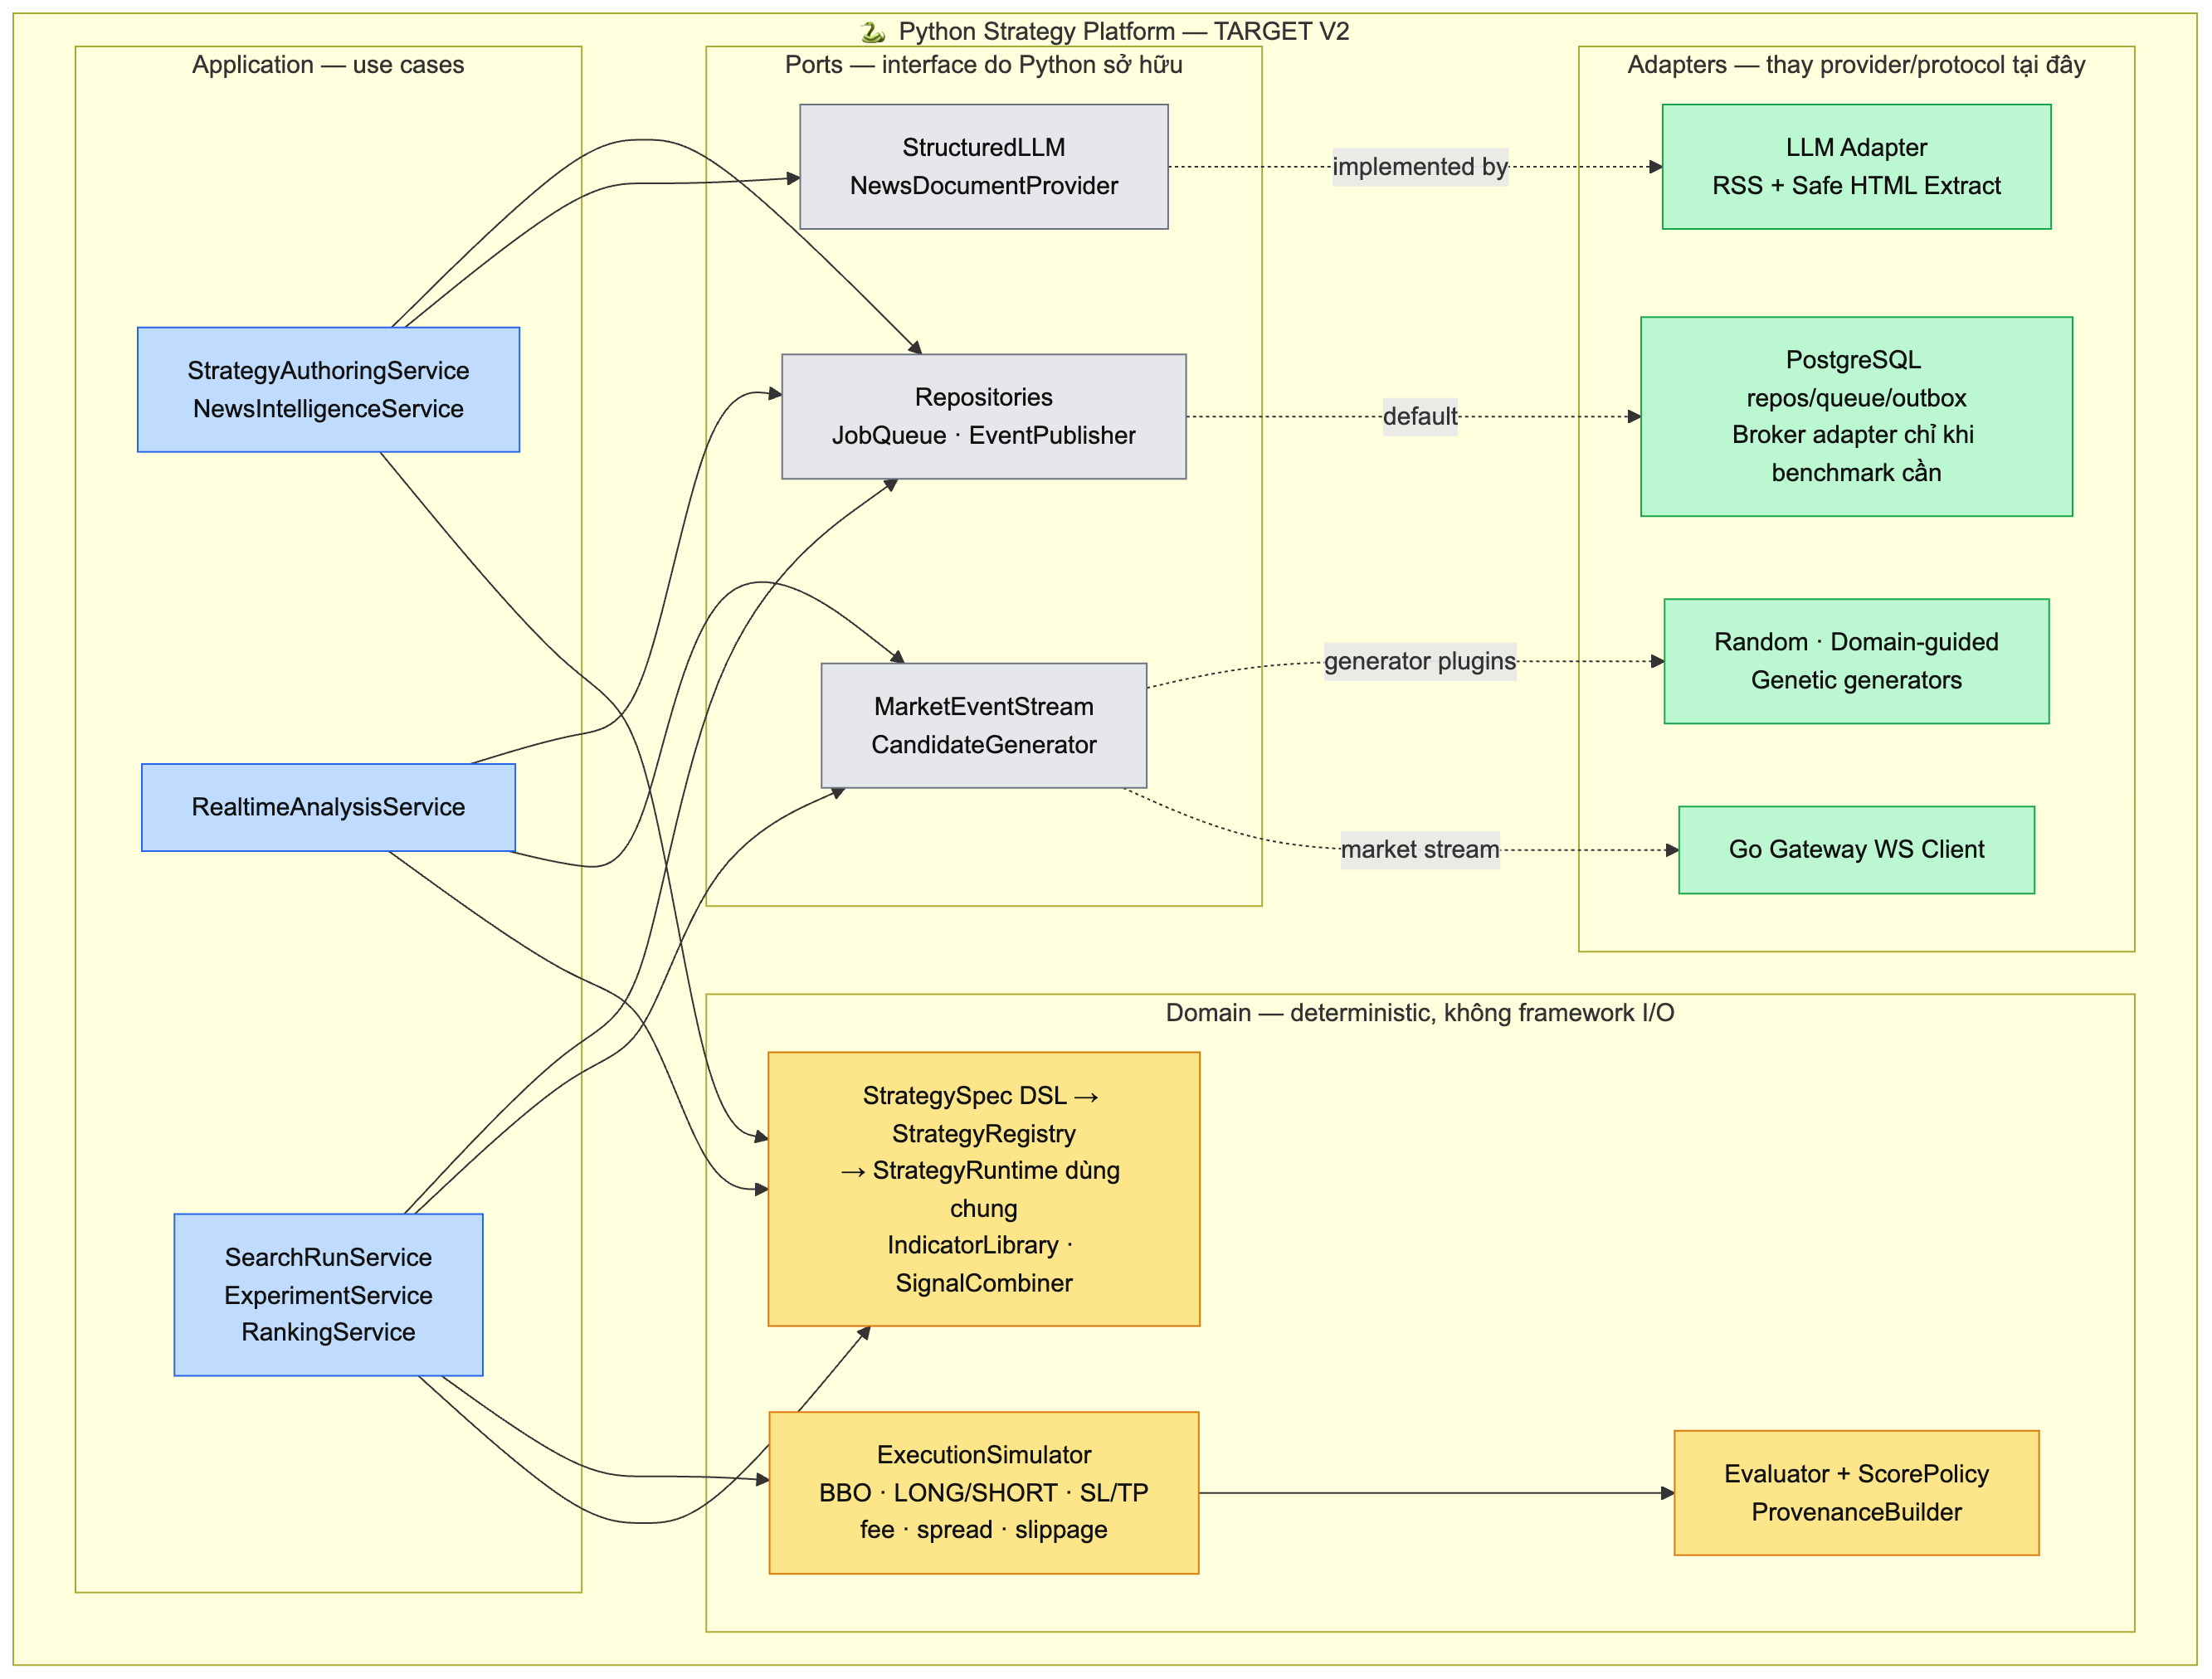
\includegraphics[width=\linewidth,height=0.75\textheight,keepaspectratio]{../blueprint/assets/diagrams-png/03-c4-l3-python-strategy-platform.png}
\end{column}
\end{columns}
\end{frame}

% Slide 10: C4 L3 Go
\begin{frame}{9. C4 Model (Level 3) - Go Edge \& Market Gateway}
\begin{columns}[c]
\begin{column}{0.45\textwidth}
\begin{itemize}
  \item \textbf{Binance Adapter:} WSS stream, tự động reconnect \& REST Backfill bù nến.
  \item \textbf{Candle Aggregator \& BBO Streamer:} Tổng hợp nến tạm \& đóng nến vào CSDL.
  \item \textbf{CQRS Request Handler:} Phân tách Command (tạo thí nghiệm) và Query (đọc nến).
  \item \textbf{Security \& Auth Middleware:} JWT token, RBAC \& Rate Limiting.
\end{itemize}
\end{column}
\begin{column}{0.53\textwidth}
\centering
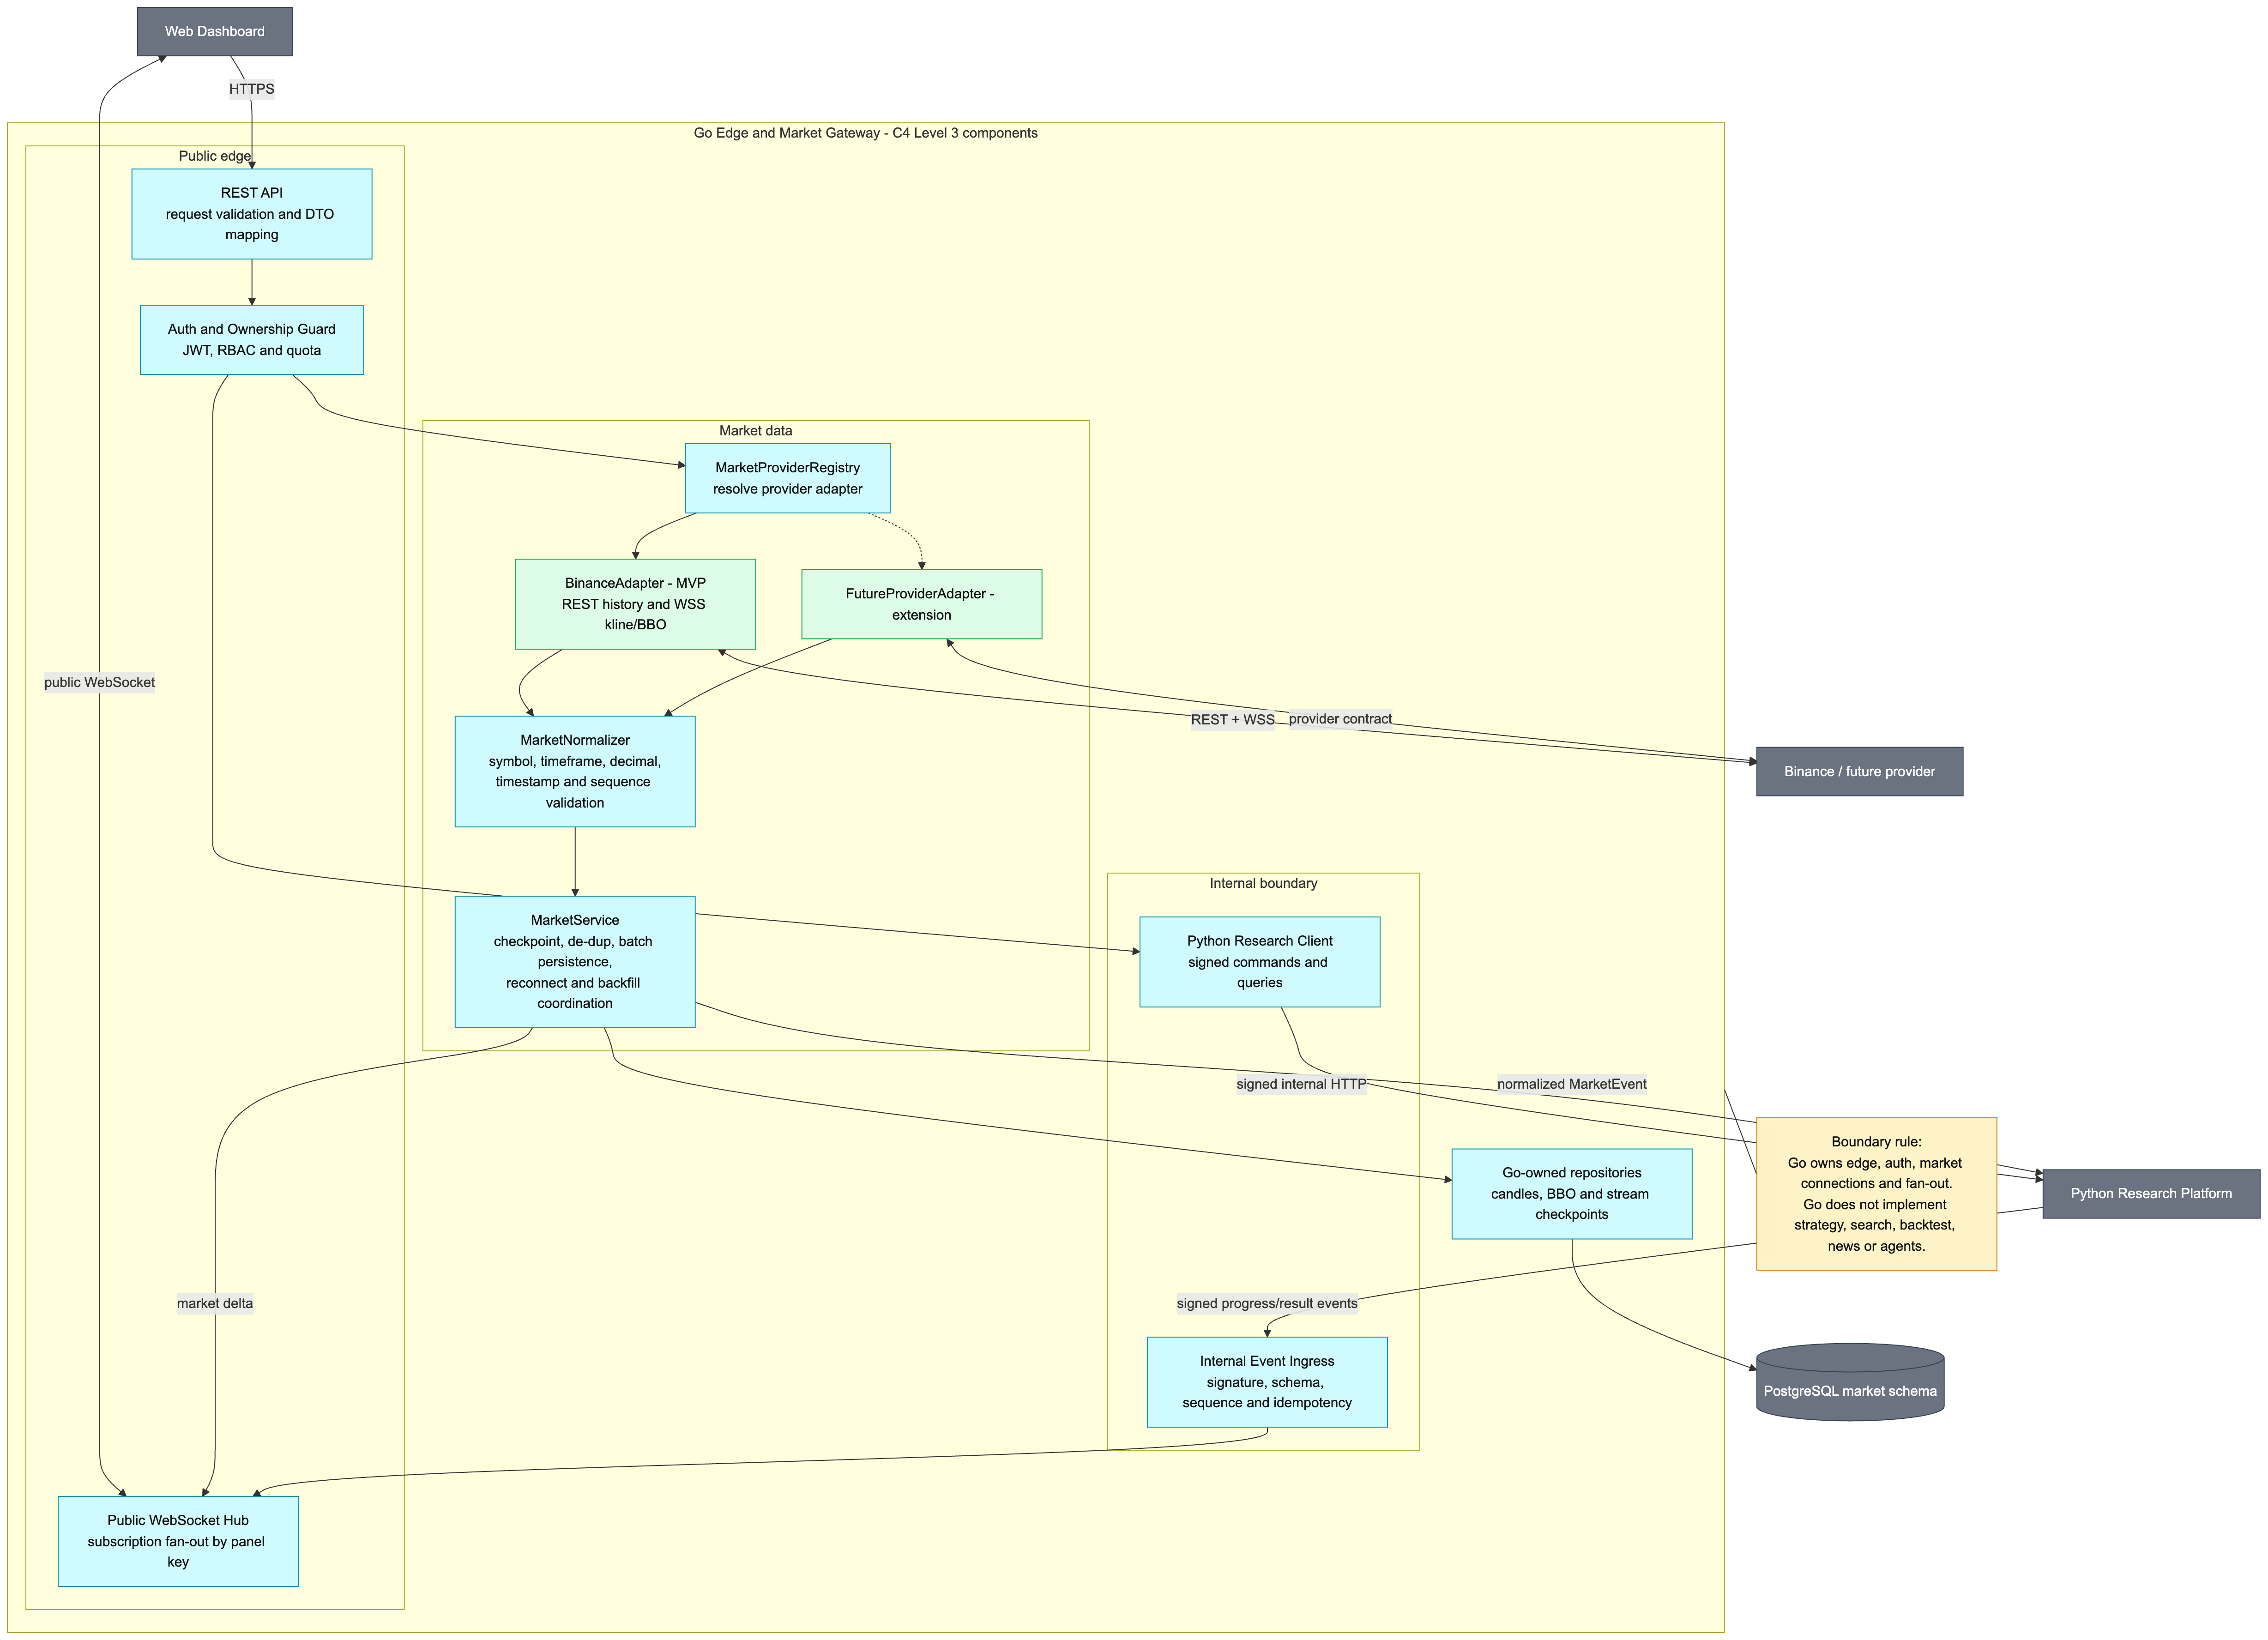
\includegraphics[width=\linewidth,height=0.75\textheight,keepaspectratio]{../blueprint/assets/diagrams-png/35-c4-l3-go-edge-market-gateway.png}
\end{column}
\end{columns}
\end{frame}

% Slide 11: Boundaries
\begin{frame}{10. Phân Định Ranh Giới 5 Module Cốt Lõi}
\begin{columns}[T]
\begin{column}{0.48\textwidth}
\begin{block}{\textbf{[5 Miền Nghiệp Vụ Chuyên Biệt]}}
\begin{enumerate}
  \item \textbf{Market Realtime (Go):} Ingestion nến, WSS, Auto-backfill.
  \item \textbf{Strategy Engine (Python):} Thực thi chiến lược, Registry.
  \item \textbf{Backtest \& Discovery (Python):} Chạy kiểm thử đa phân vùng (Train/Val/Test).
  \item \textbf{News Crawler (Python):} Thu thập RSS/HTML, SSRF guard.
  \item \textbf{News Intelligence (AI):} Phân tích sentiment độc lập.
\end{enumerate}
\end{block}
\end{column}
\begin{column}{0.48\textwidth}
\begin{block}{\textbf{[Language Boundary]}}
\resizebox{\linewidth}{!}{%
\begin{tabular}{lp{2.4cm}p{2.6cm}}
\toprule
\textbf{Tiêu chí} & \textbf{Go Edge} & \textbf{Python Engine} \\
\midrule
\textbf{Sở hữu} & Market Ingestion, API & Backtest, Strategy, AI \\
\textbf{Thế mạnh} & Goroutines, Low RAM & Vectorization, AST, ML \\
\textbf{Giao thức} & REST CQRS, WSS & Worker Queue Leases \\
\textbf{Cô lập lỗi} & Sàn lỗi không chết Worker & Crash thuật toán không nghẽn API \\
\bottomrule
\end{tabular}}
\end{block}
\end{column}
\end{columns}
\end{frame}

% Slide 12: Module Specs
\begin{frame}{11. Đặc Tả Ranh Giới \& Phạm Vi Từng Module}
\begin{columns}[T]
\begin{column}{0.48\textwidth}
\begin{block}{\textbf{[1. Market Realtime \& 2. Strategy Engine]}}
\begin{itemize}
  \item \textbf{Market Realtime:} Input là raw WSS stream; Output là normalized \texttt{Candle} \& \texttt{BBO}; Invariant: không duplicate nến.
  \item \textbf{Strategy Engine:} Input là \texttt{StrategyContext}; Output là \texttt{Signal} (\texttt{BUY/SELL/HOLD}); Độc lập hoàn toàn với nguồn dữ liệu.
\end{itemize}
\end{block}
\end{column}
\begin{column}{0.48\textwidth}
\begin{block}{\textbf{[3. Backtest, 4. Crawler \& 5. Intelligence]}}
\begin{itemize}
  \item \textbf{Backtest \& Discovery:} Input là \texttt{ExperimentConfig}; Output là \texttt{BacktestResult} kèm Provenance Hash.
  \item \textbf{News Crawler \& Intelligence:} Thu thập tin an toàn SSRF; Chấm điểm \texttt{SentimentResult} [-1.0, 1.0] bất đồng bộ.
\end{itemize}
\end{block}
\end{column}
\end{columns}
\end{frame}

% Slide 13: UML Strategy
\begin{frame}{12. UML Class Diagram: Strategy Plugin Model}
\begin{columns}[c]
\begin{column}{0.45\textwidth}
\begin{itemize}
  \item \textbf{Contract \texttt{IStrategy}:} \texttt{evaluate(context) -> Signal}.
  \item \textbf{5 Core Strategies:} \texttt{ma\_crossover}, \texttt{bollinger\_bands}, \texttt{rsi\_threshold}, \texttt{smc\_structure}, \texttt{news\_sentiment}.
  \item \textbf{Composite Strategy:} Tổ hợp 2-5 chiến lược con với \texttt{CombinationPolicy} (majority/weighted).
  \item \textbf{Strategy Registry:} Dynamic load plugin không cần compile lại.
\end{itemize}
\end{column}
\begin{column}{0.53\textwidth}
\centering
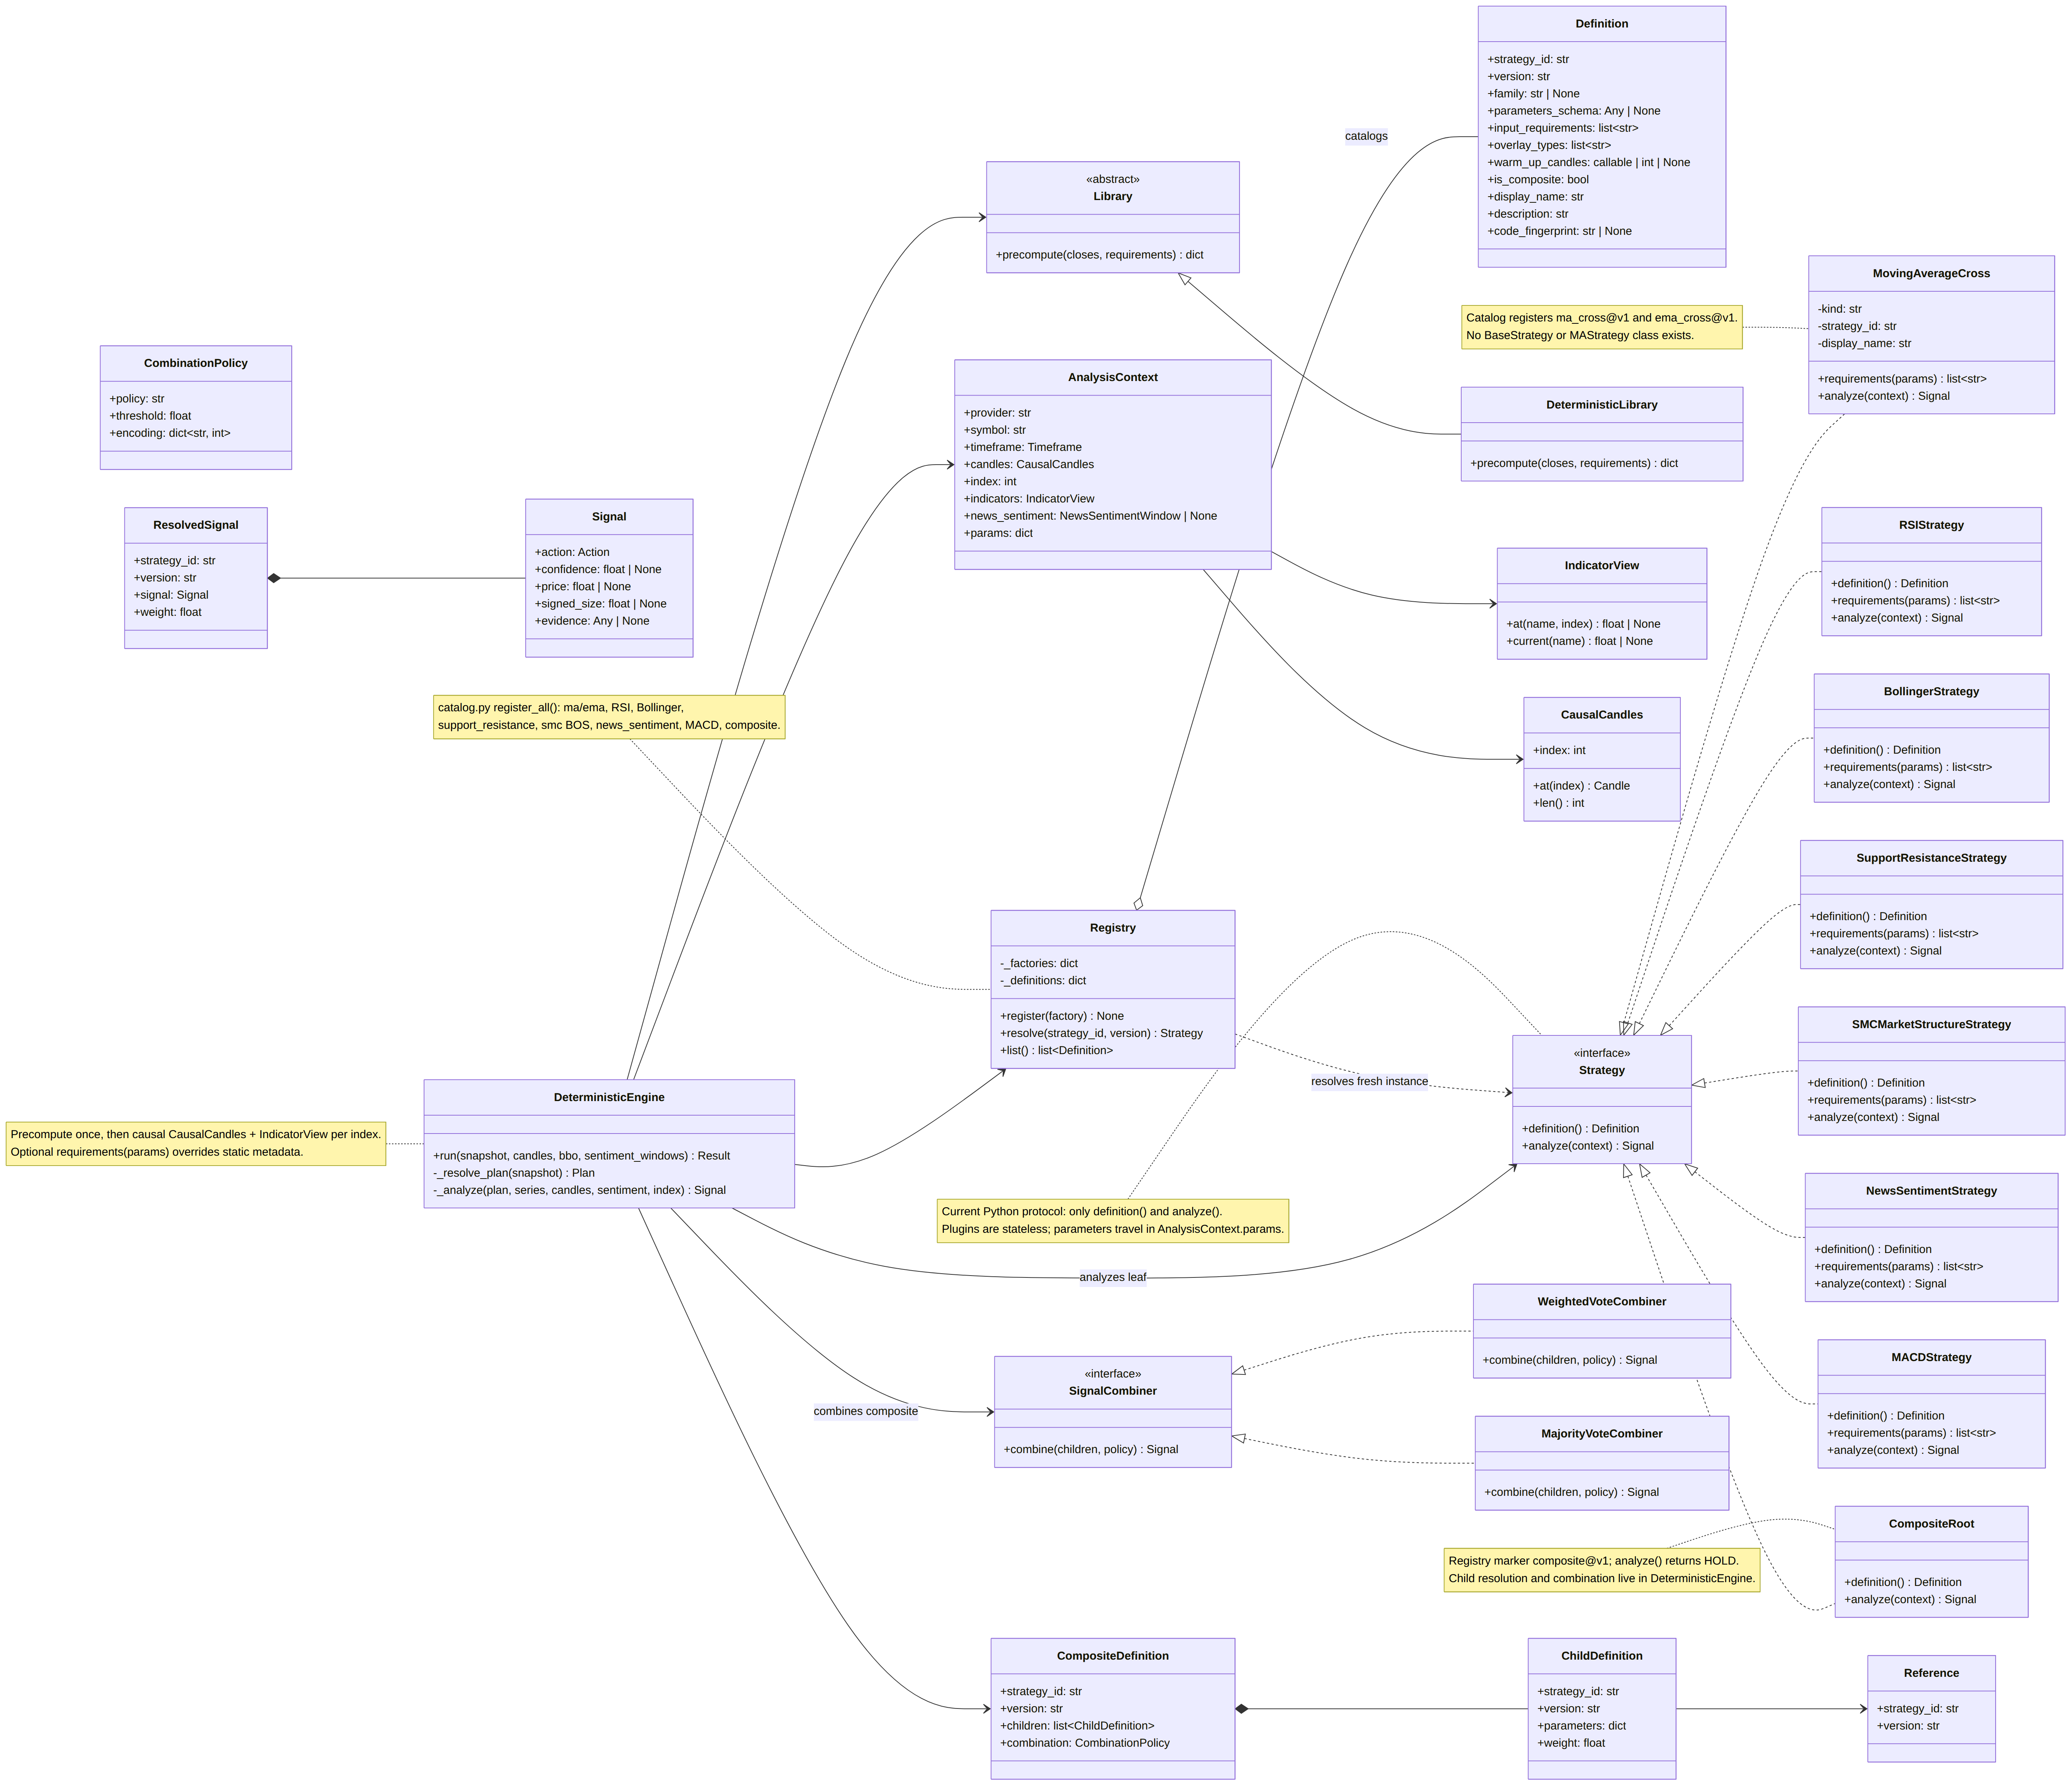
\includegraphics[width=\linewidth,height=0.75\textheight,keepaspectratio]{../blueprint/assets/diagrams-png/36-uml-strategy-plugin-model.png}
\end{column}
\end{columns}
\end{frame}

% Slide 14: UML Search
\begin{frame}{13. UML Class Diagram: Search Algorithm \& Discovery}
\begin{columns}[c]
\begin{column}{0.45\textwidth}
\begin{itemize}
  \item \textbf{Contract \texttt{ISearchAlgorithm}:} RandomSearch, GeneticAlgorithm, BayesianOptimization.
  \item \textbf{3-Stage Discovery (Chống Overfitting):}
  \begin{itemize}
    \item \textbf{Train (30d):} Tìm kiếm biến thể.
    \item \textbf{Validation (15d):} Kiểm tra tổng quát.
    \item \textbf{Sealed Test (15d):} Đánh giá độc lập trước Leaderboard.
  \end{itemize}
  \item \textbf{Idempotency:} Trial Reservation chống tạo job tràn lan.
\end{itemize}
\end{column}
\begin{column}{0.53\textwidth}
\centering
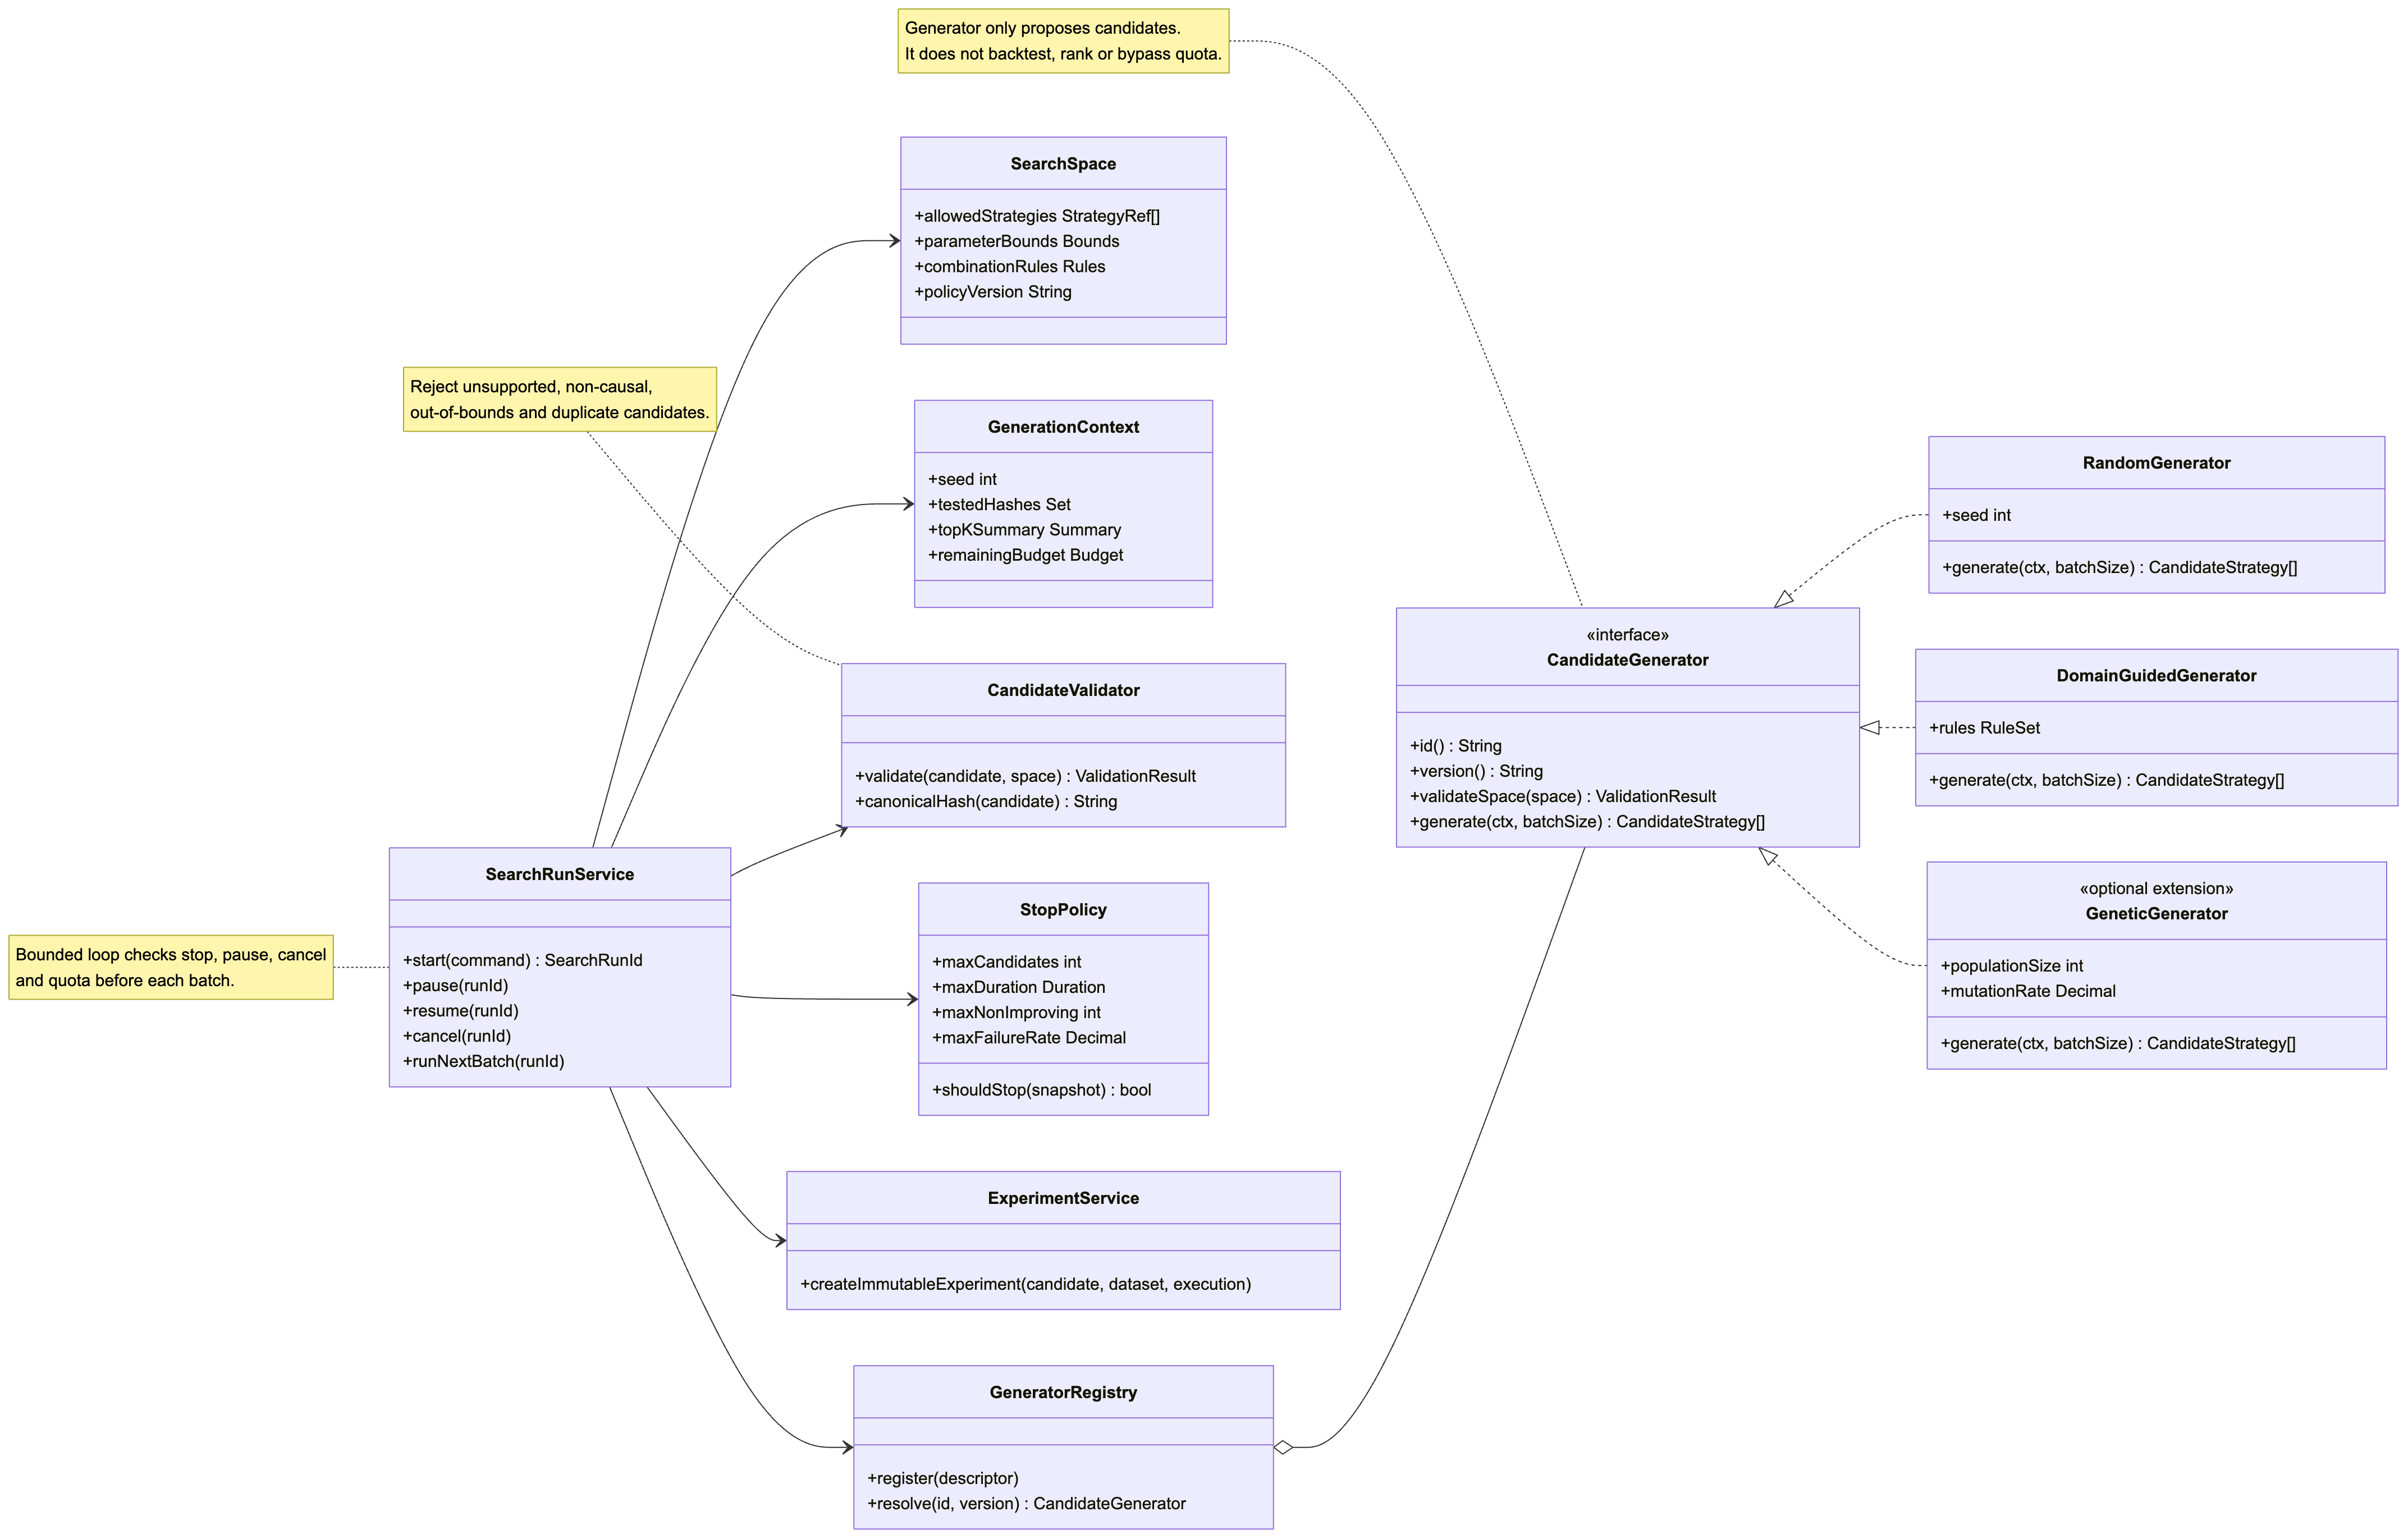
\includegraphics[width=\linewidth,height=0.75\textheight,keepaspectratio]{../blueprint/assets/diagrams-png/37-uml-search-algorithm-model.png}
\end{column}
\end{columns}
\end{frame}

% Slide 15: UML News
\begin{frame}{14. UML Class Diagram: Resilient News Crawler}
\begin{columns}[c]
\begin{column}{0.45\textwidth}
\begin{itemize}
  \item \textbf{Contract \texttt{NewsProvider}:} \texttt{RssNewsProvider} \& \texttt{HtmlNewsProvider}.
  \item \textbf{Chốt chặn an toàn SSRF:} Resolver \& Fetcher kiểm tra DNS, private IP, redirect limit.
  \item \textbf{Quality Gate \& LLM Fallback:} Kích hoạt \texttt{NewsExtractionHTTPAdapter} khi HTML đổi cấu trúc.
  \item \textbf{Tách biệt Crawler \& Sentiment:} AI lỗi không làm gián đoạn thu thập tin.
\end{itemize}
\end{column}
\begin{column}{0.53\textwidth}
\centering
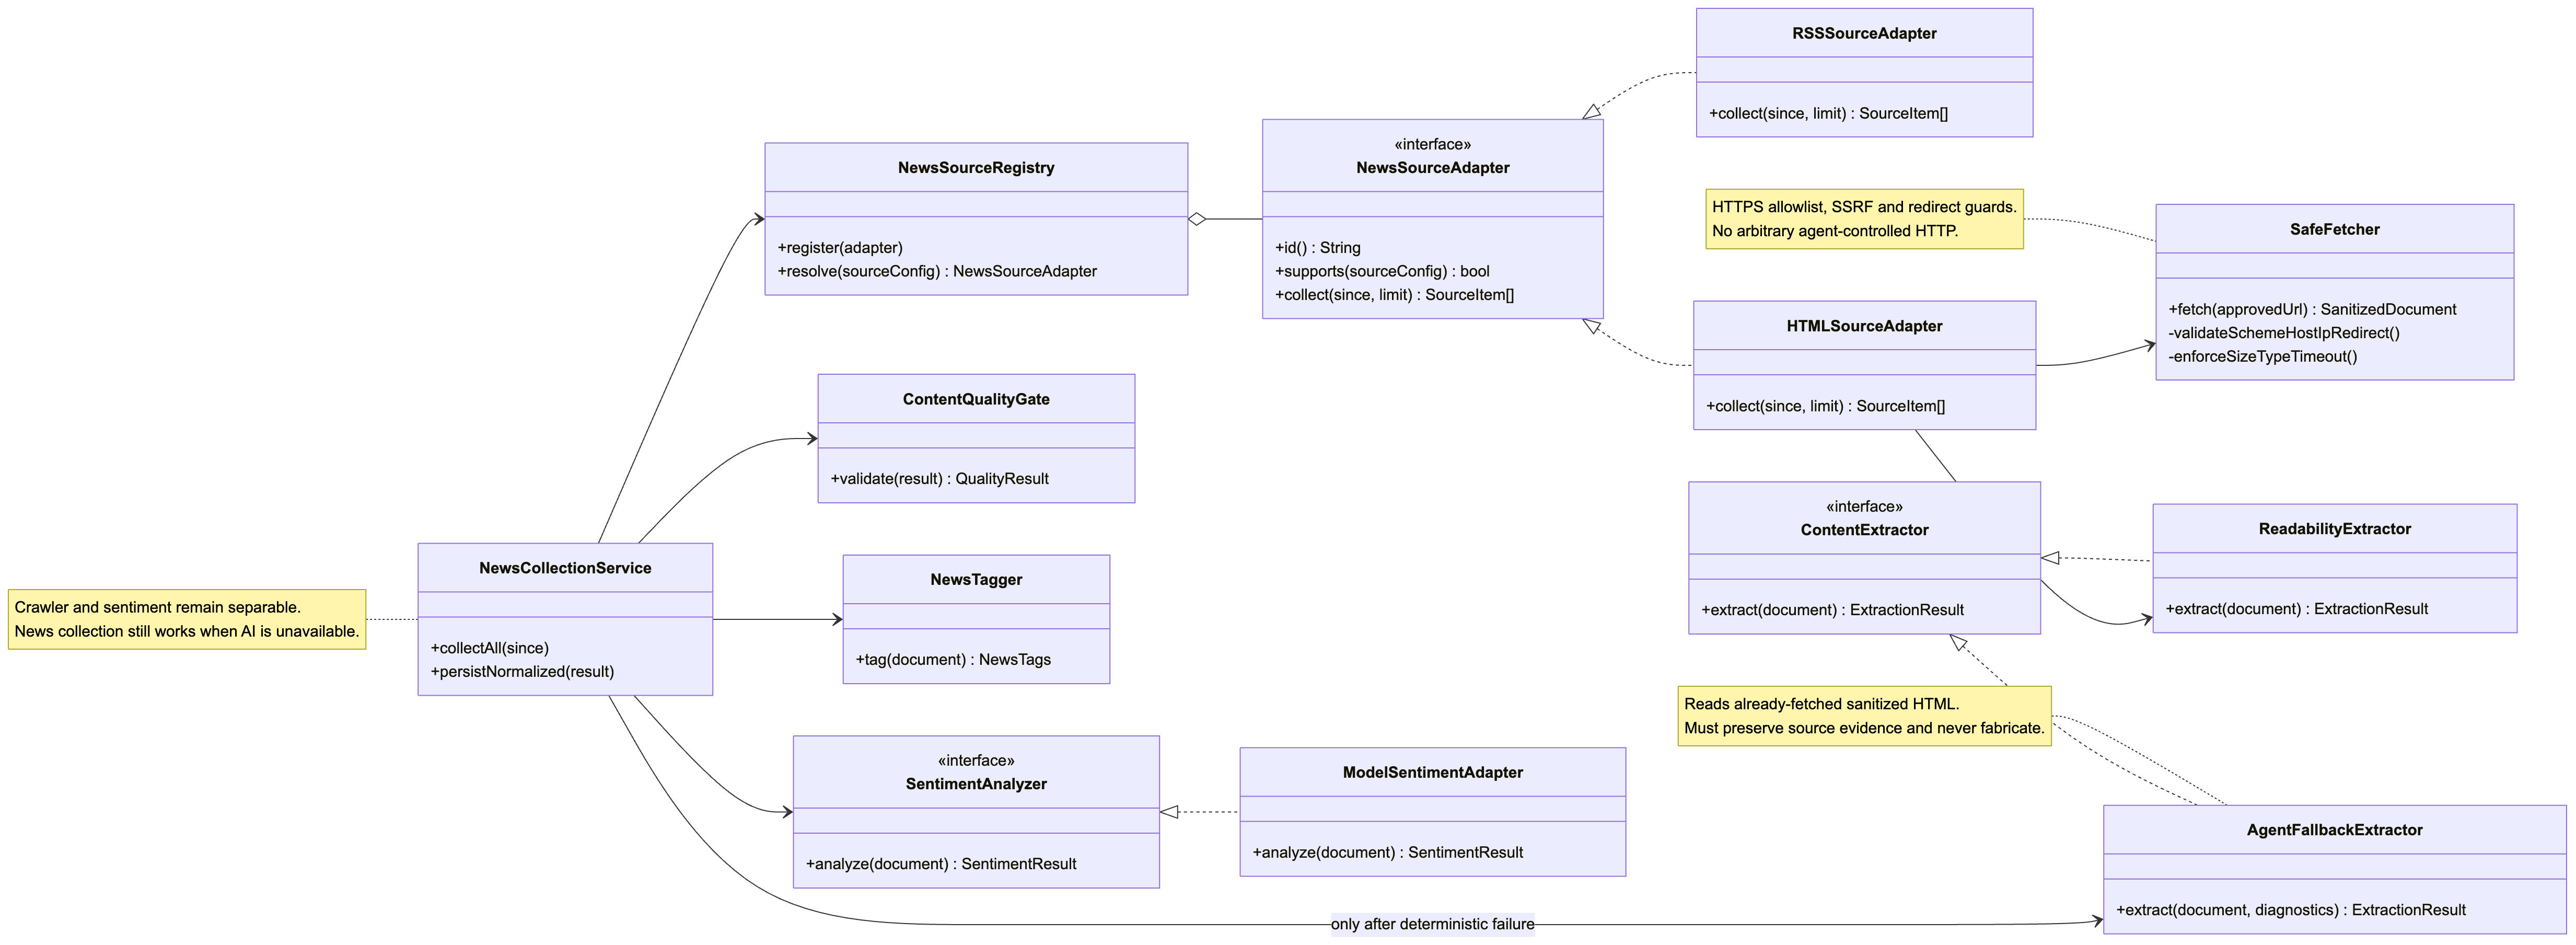
\includegraphics[width=\linewidth,height=0.75\textheight,keepaspectratio]{../blueprint/assets/diagrams-png/38-uml-news-crawler-model.png}
\end{column}
\end{columns}
\end{frame}

% Slide 16: High-Level Architecture
\begin{frame}{15. High-Level Architecture: Modular Monolith + Async Workers}
\begin{columns}[c]
\begin{column}{0.45\textwidth}
\begin{itemize}
  \item \textbf{Frontend Layer:} Next.js SPA qua REST CQRS \& SSE/WebSocket.
  \item \textbf{API \& Edge (Go):} Tiếp nhận request, RBAC, WSS Binance, SSE broadcaster.
  \item \textbf{Research Core (Python):} Worker Pool xử lý Backtest, Discovery Loop, Genetic Search.
  \item \textbf{Storage \& Outbox:} PostgreSQL ACID Outbox \& In-memory Ring Buffers.
\end{itemize}
\end{column}
\begin{column}{0.53\textwidth}
\centering

\includegraphics[width=\linewidth,height=0.75\textheight,keepaspectratio]{../blueprint/assets/diagrams-png/04-high-level-architecture.png}
\end{column}
\end{columns}
\end{frame}

% Slide 17: Design Patterns
\begin{frame}{16. Các Design \& Architectural Patterns Trọng Yếu}
\begin{columns}[c]
\begin{column}{0.45\textwidth}
\begin{itemize}
  \item \textbf{CQRS:} Phân tách luồng Command (ghi thí nghiệm) và Query (đọc nến, leaderboard).
  \item \textbf{Transactional Outbox:} Atomic transaction đảm bảo không mất mát job thực thi.
  \item \textbf{Dual-Channel Parity:} Đồng nhất schema cho Realtime WSS và Historical Backfill.
  \item \textbf{Plugin Architecture:} Độc lập hóa thuật toán giao dịch khỏi execution core.
\end{itemize}
\end{column}
\begin{column}{0.53\textwidth}
\centering
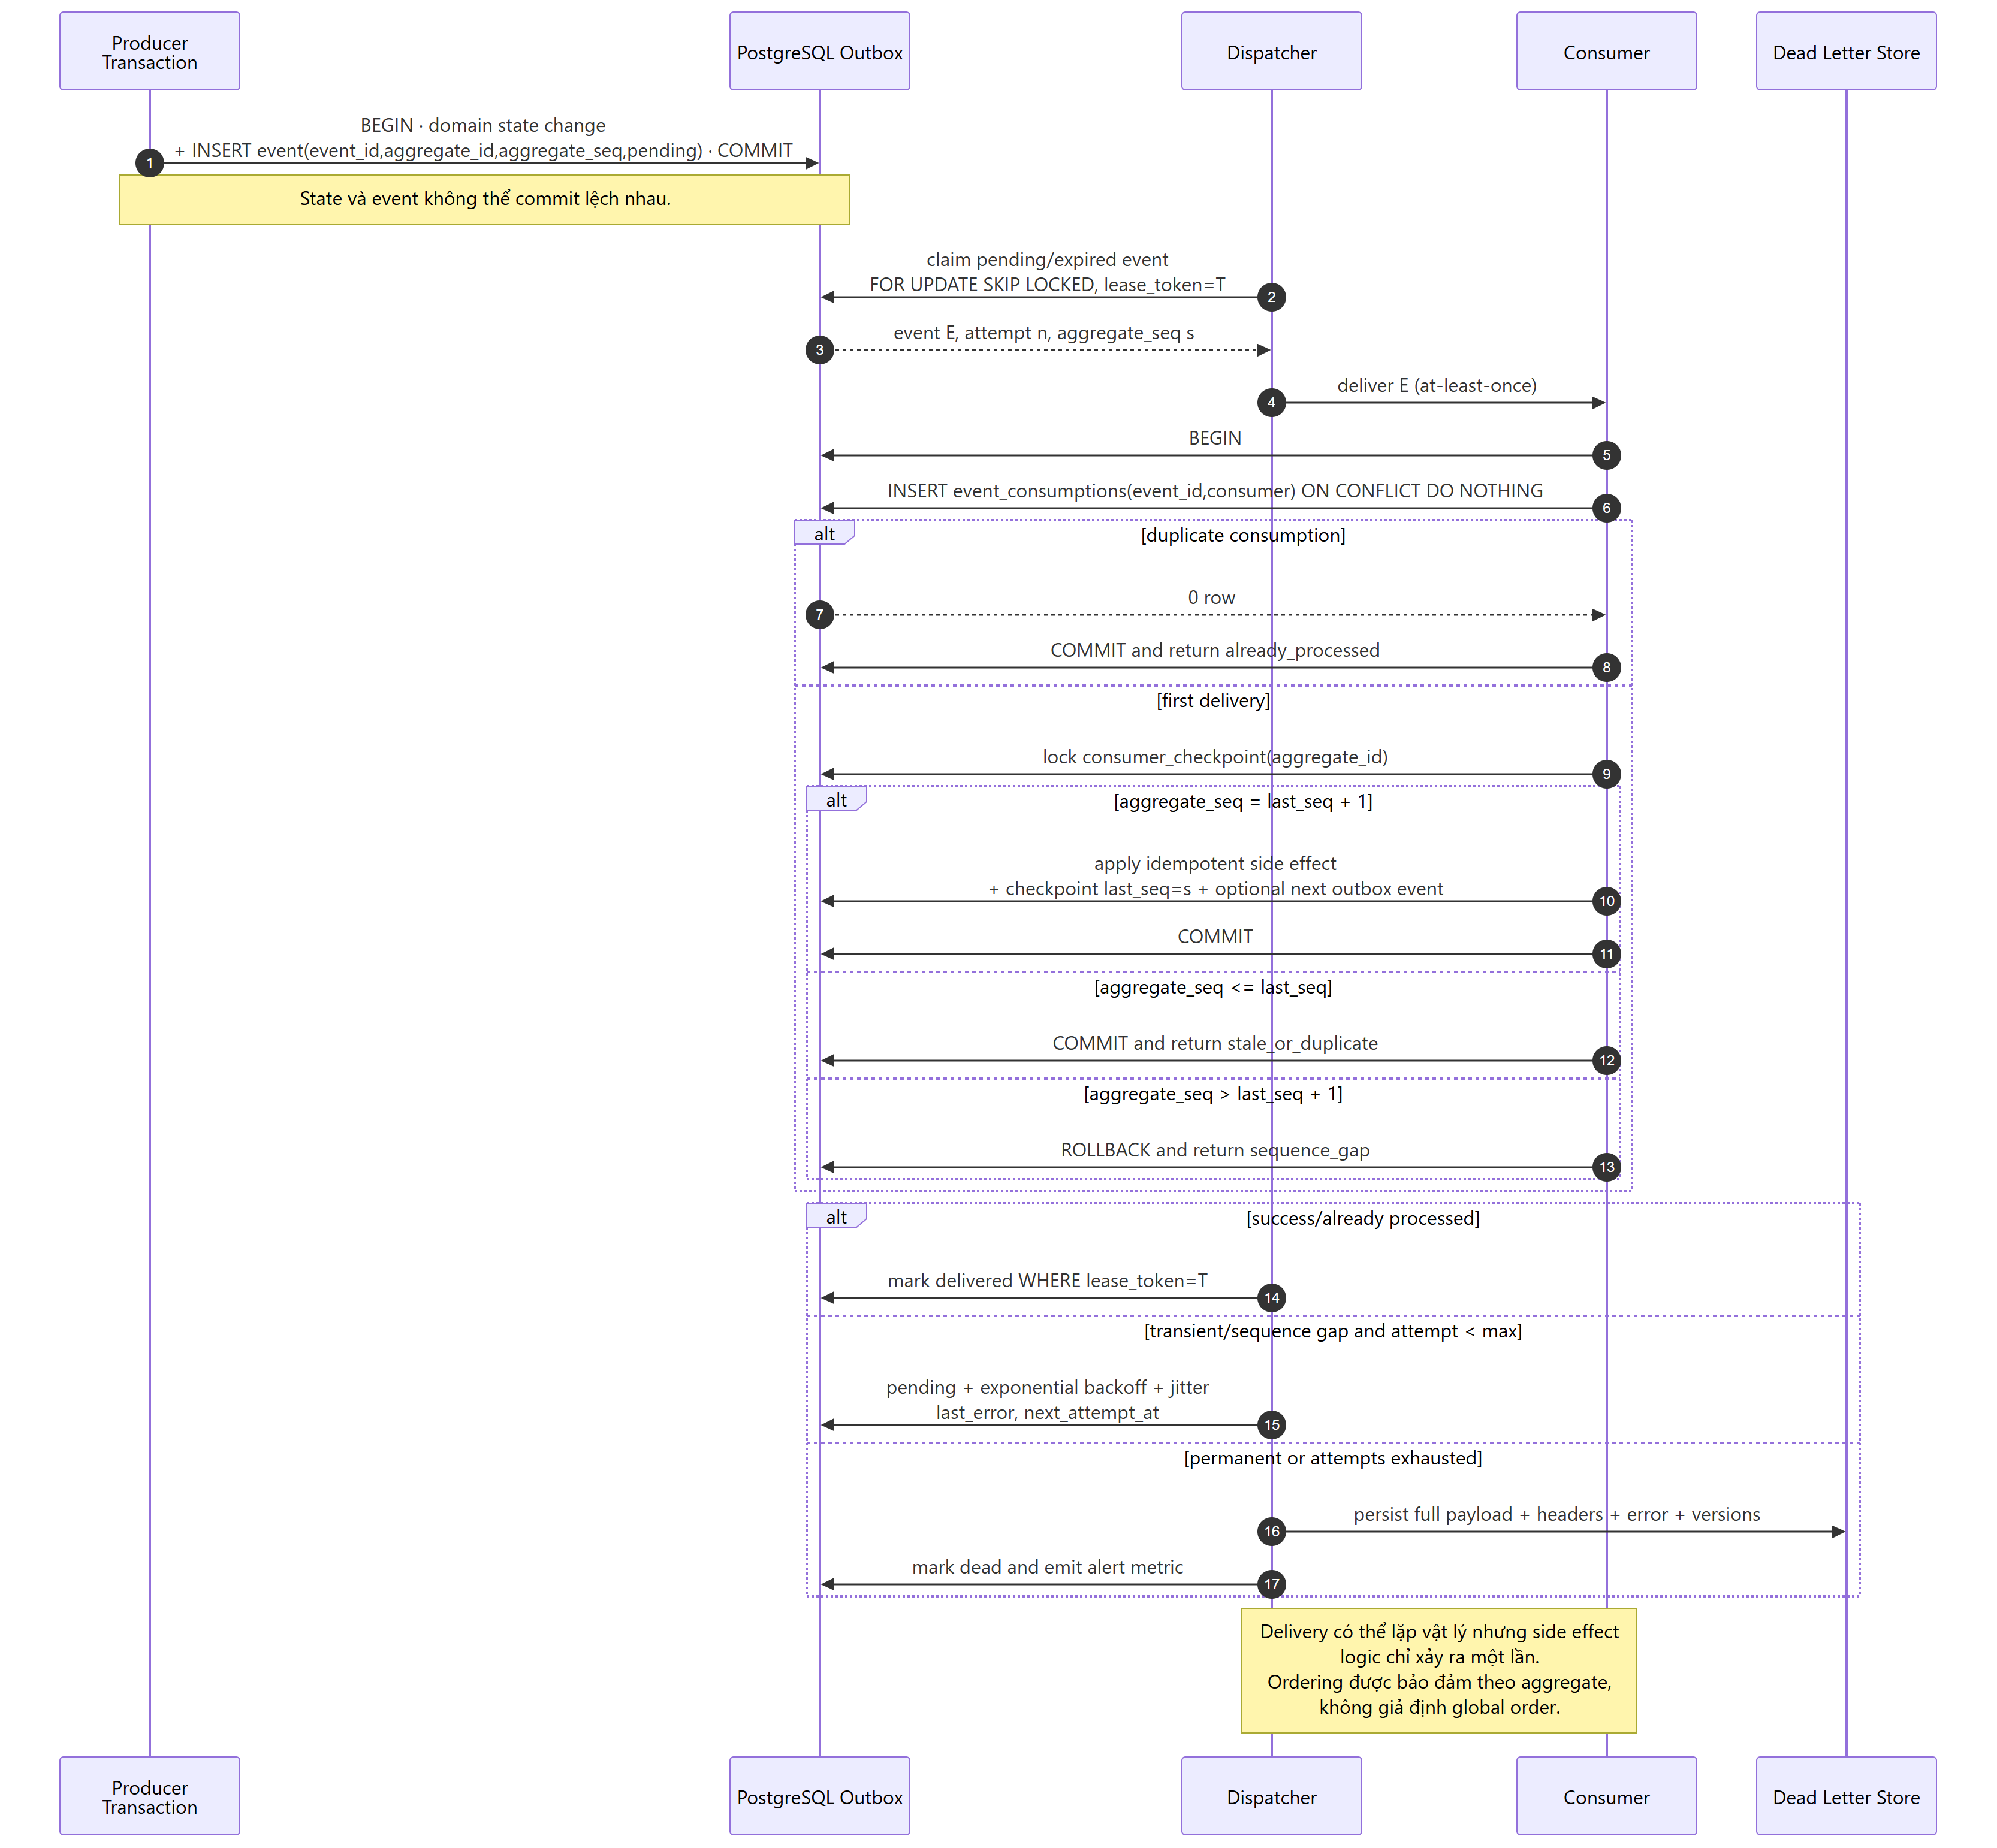
\includegraphics[width=\linewidth,height=0.75\textheight,keepaspectratio]{../blueprint/assets/diagrams-png/07-outbox-retry-order.png}
\end{column}
\end{columns}
\end{frame}

% Slide 18: Multi-Agent
\begin{frame}{17. Nền Tảng Multi-Agent \& Vòng Lặp AI Tự Chủ}
\begin{columns}[c]
\begin{column}{0.45\textwidth}
\begin{itemize}
  \item \textbf{Strategy Designer Agent:} Nhận prompt tự nhiên $\rightarrow$ sinh JSON Draft.
  \item \textbf{Implementation Agent:} Sinh Python code tuân thủ \texttt{IStrategy}.
  \item \textbf{Self-Repair Loop (AST + Sandbox):} Chạy thử trong sandbox, tự sửa code khi lỗi (tối đa 3 lần).
  \item \textbf{Candidate Discovery Agent:} Tự động biến đổi tham số và xếp hạng Leaderboard.
\end{itemize}
\end{column}
\begin{column}{0.53\textwidth}
\centering
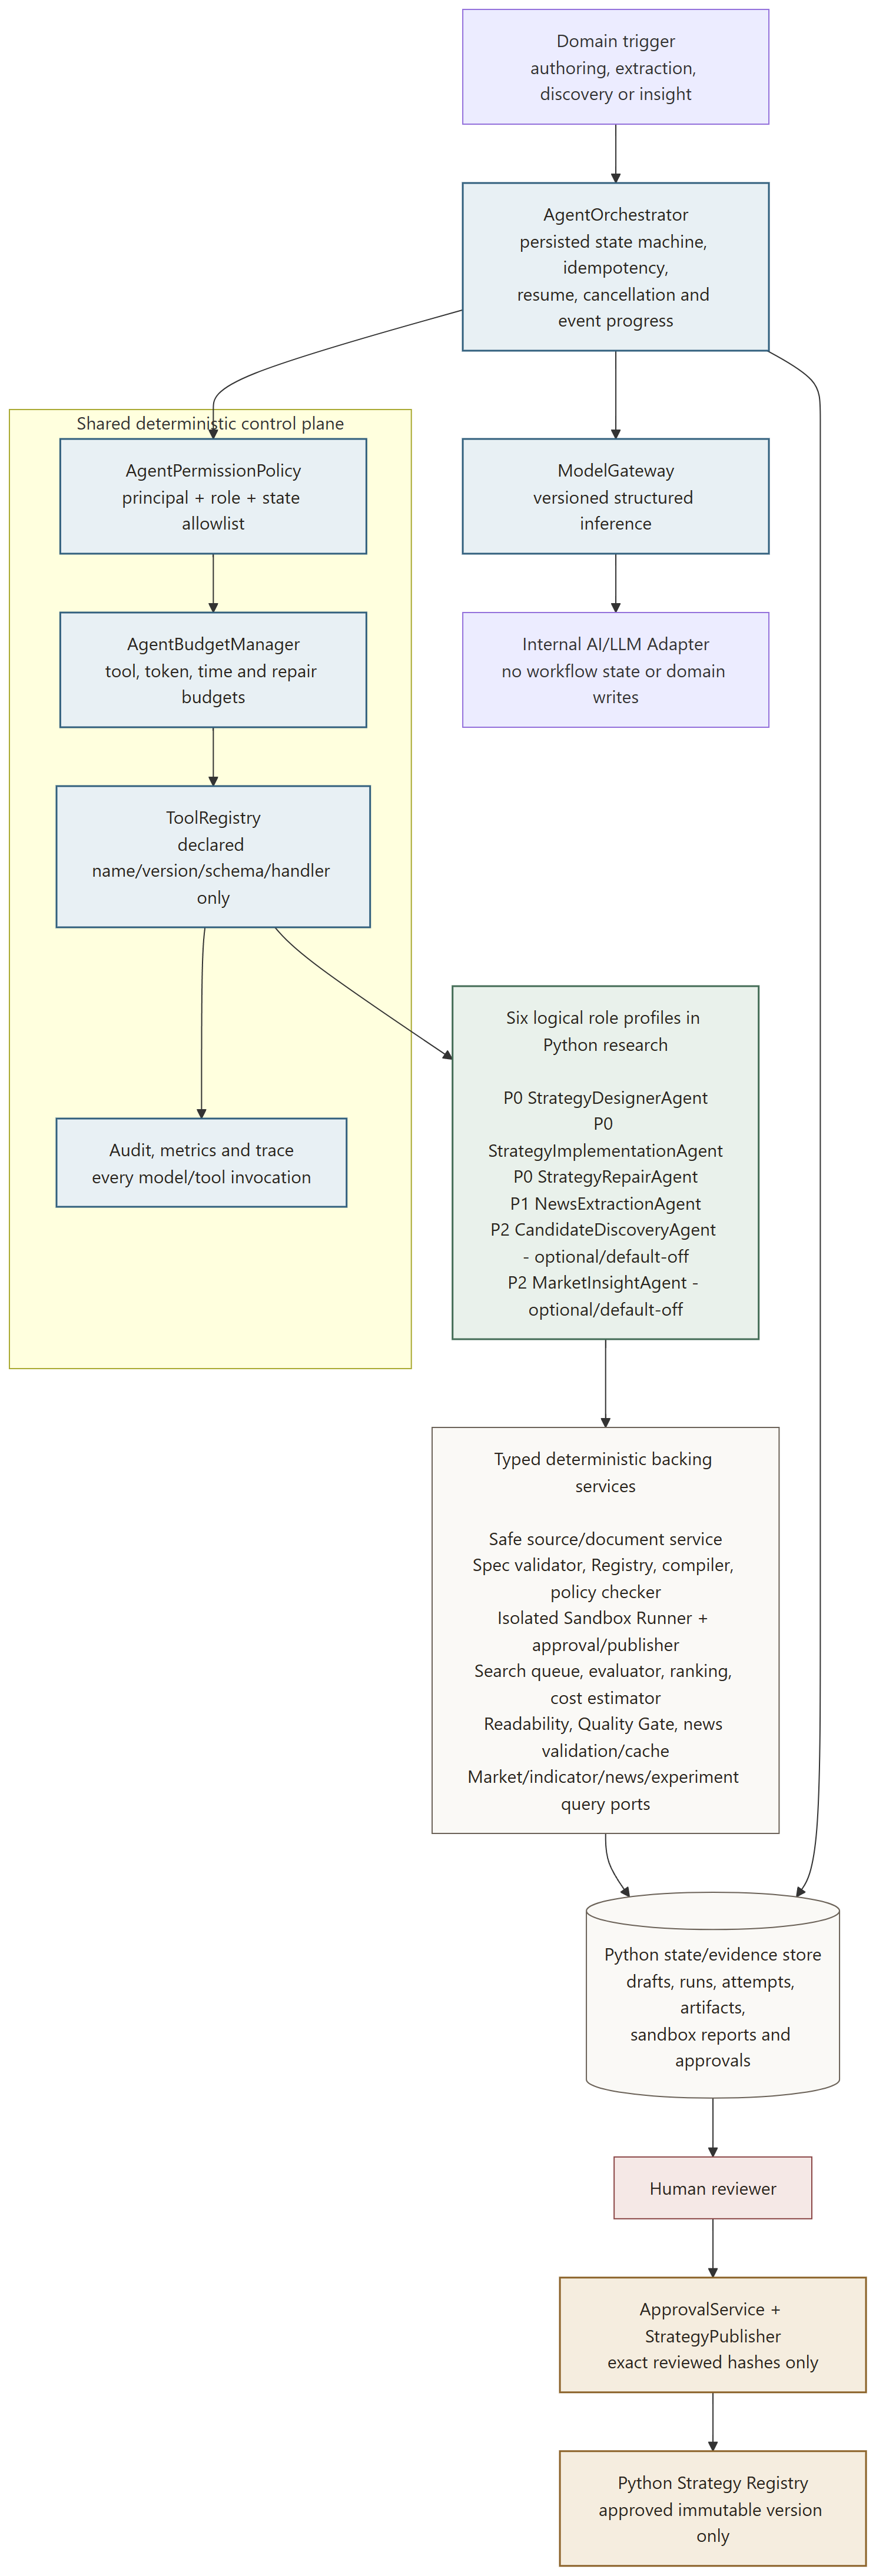
\includegraphics[width=\linewidth,height=0.75\textheight,keepaspectratio]{../blueprint/assets/diagrams-png/25-agent-platform-components.png}
\end{column}
\end{columns}
\end{frame}

% Slide 19: Realtime Reconnect Flow
\begin{frame}{18. Runtime Flow: Luồng Nạp Nến Realtime \& Tự Phục Hồi}
\begin{columns}[c]
\begin{column}{0.45\textwidth}
\begin{enumerate}
  \item \textbf{Bootstrap:} Tải 1,000 nến lịch sử cho các khung 1m, 5m, 1h, 1d.
  \item \textbf{WSS Stream:} Tiếp nhận ticker \& cập nhật nến tạm thời.
  \item \textbf{Candle Close:} Ghi nến vào Postgres, bắn sự kiện \texttt{CandleClosed}.
  \item \textbf{Reconnect \& Backfill:} Khi rớt mạng WSS, tự động kéo bù nến qua REST API.
\end{enumerate}
\end{column}
\begin{column}{0.53\textwidth}
\centering
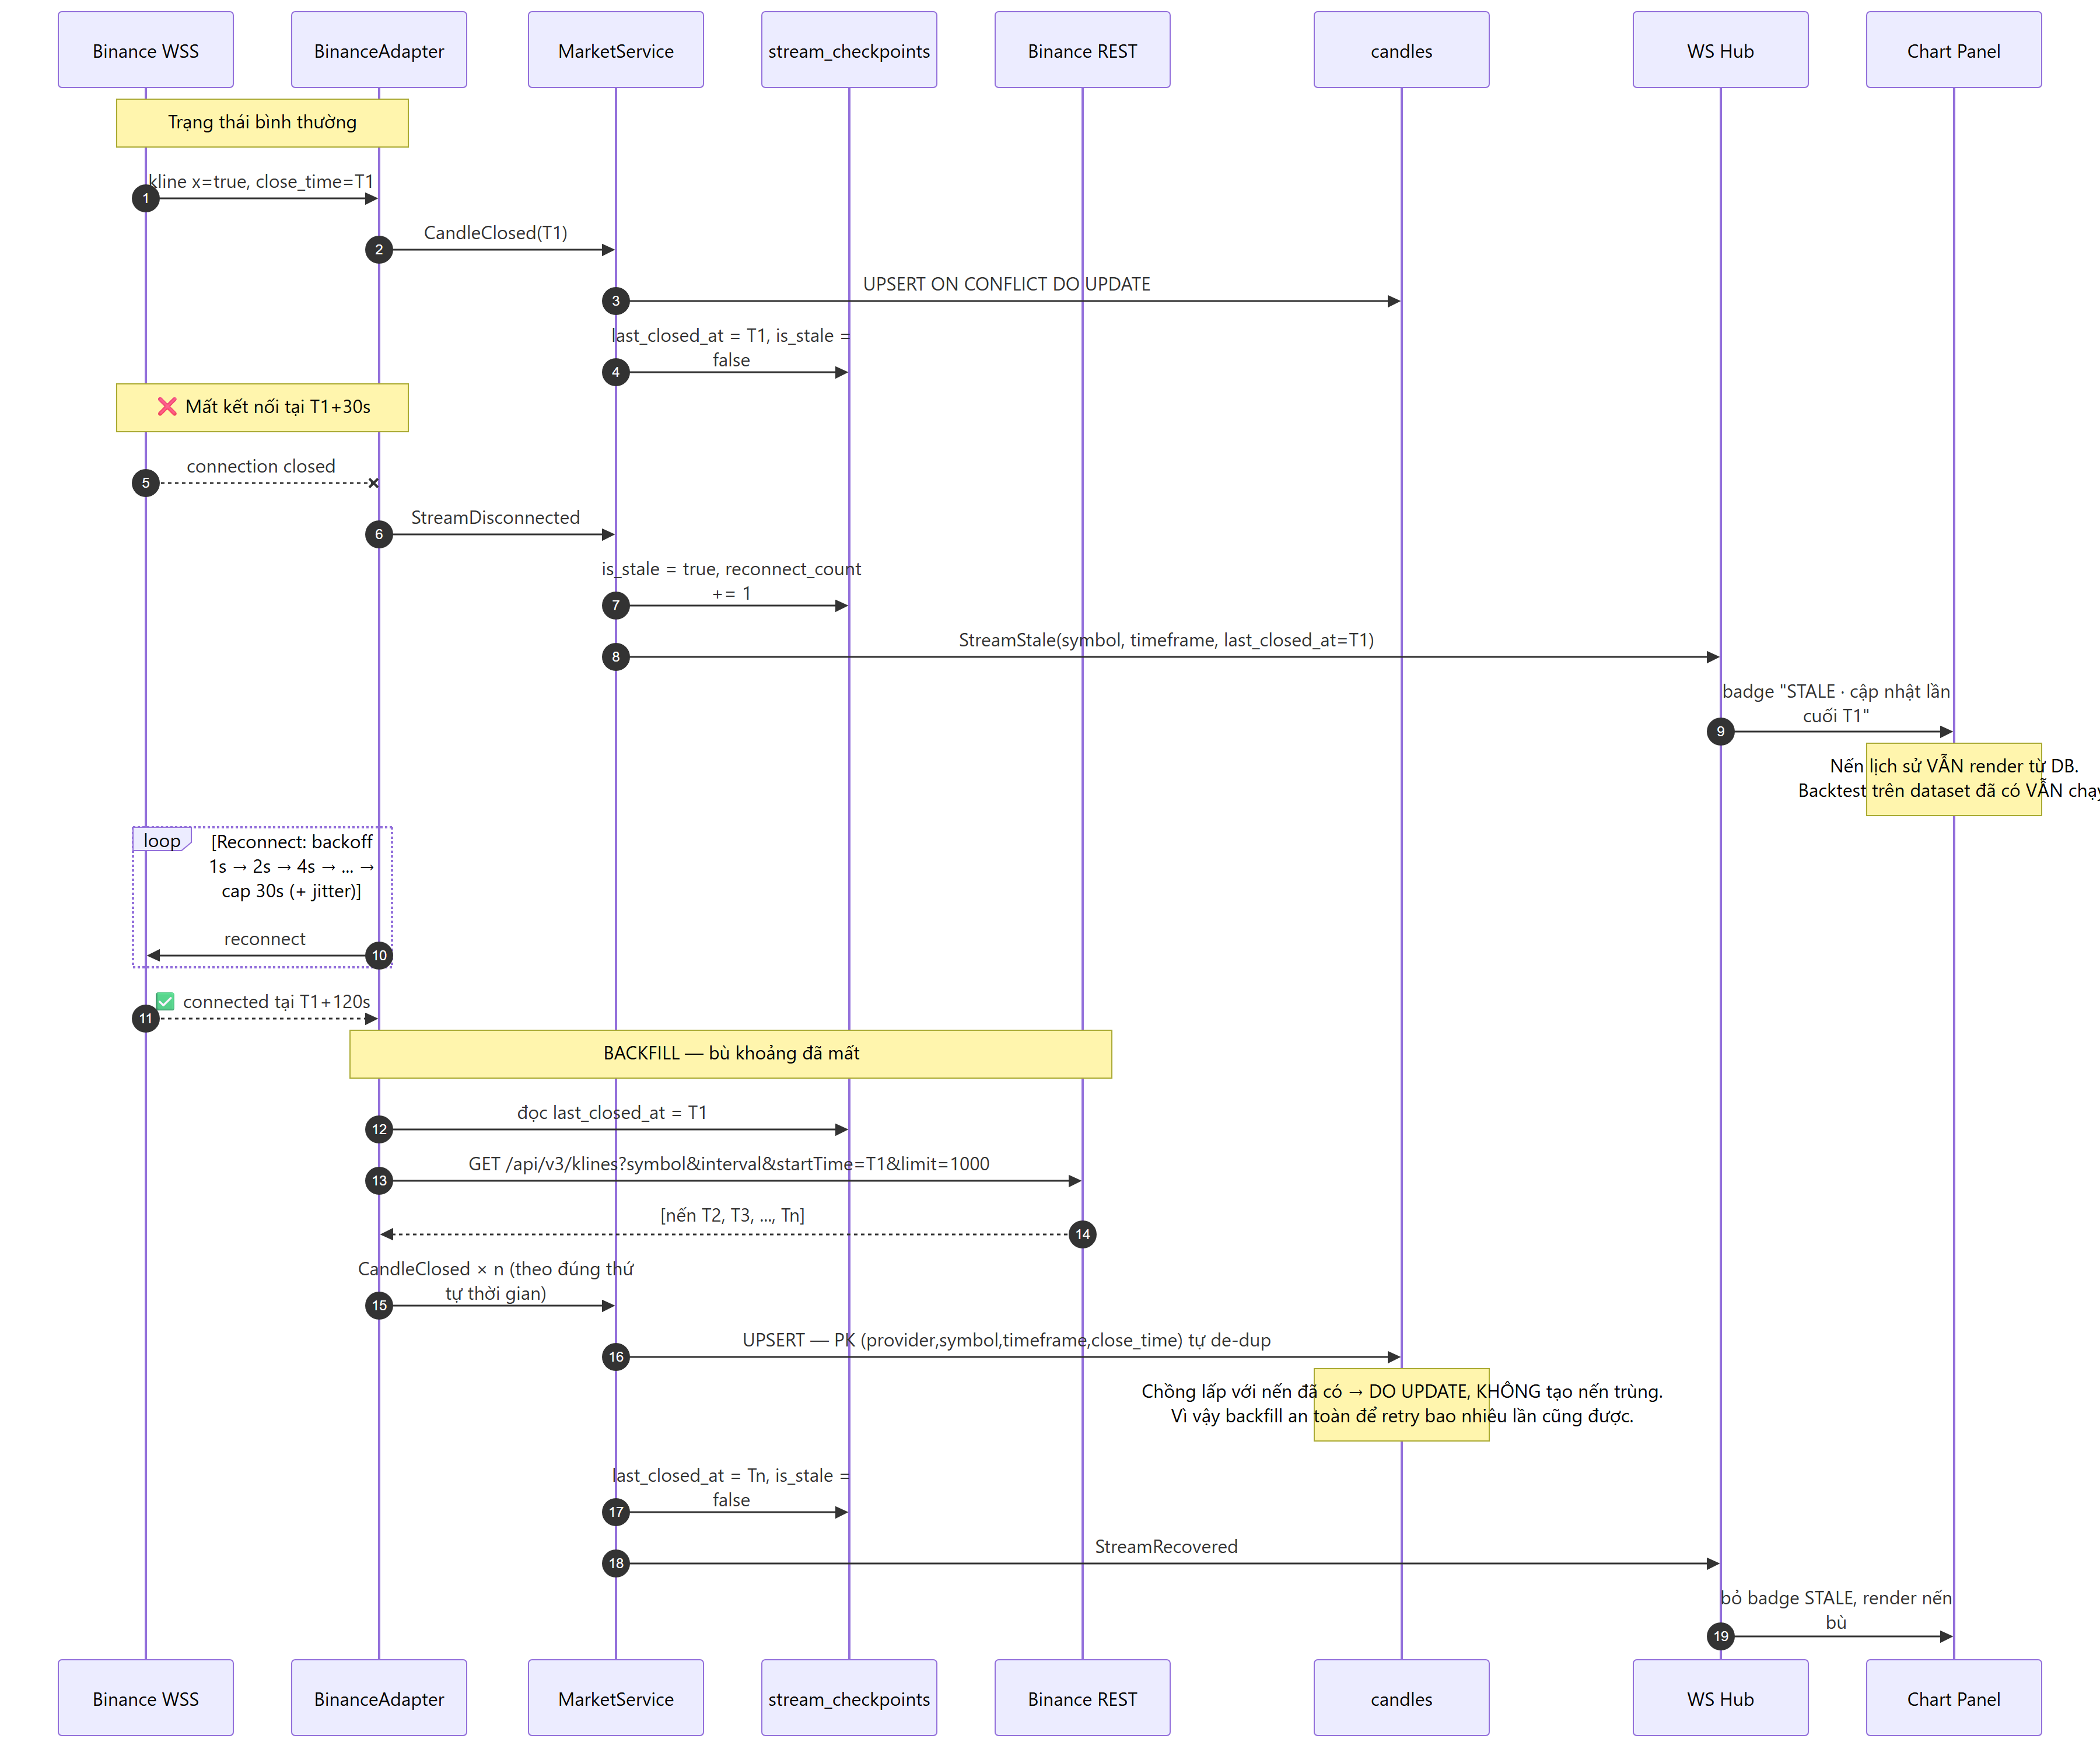
\includegraphics[width=\linewidth,height=0.75\textheight,keepaspectratio]{../blueprint/assets/diagrams-png/09-realtime-reconnect-backfill-flow.png}
\end{column}
\end{columns}
\end{frame}

% Slide 20: Strategy Flow
\begin{frame}{19. Runtime Flow: Thực Thi Chiến Lược \& Parity}
\begin{columns}[c]
\begin{column}{0.45\textwidth}
\begin{itemize}
  \item \textbf{Thực thi Chiến lược (\texttt{10-strategy-flow}):}
  \begin{itemize}
    \item Nạp \texttt{Datafeed} \& \texttt{Sentiment} vào \texttt{StrategyContext}.
    \item \texttt{IStrategy.evaluate()} sinh tín hiệu BUY/SELL/HOLD.
    \item \texttt{CompositeStrategy} tổng hợp tín hiệu trọng số.
  \end{itemize}
  \item \textbf{Runtime Parity:} Cùng 1 interface và schema dữ liệu trên cả Live data và Historical Backtest.
\end{itemize}
\end{column}
\begin{column}{0.53\textwidth}
\centering
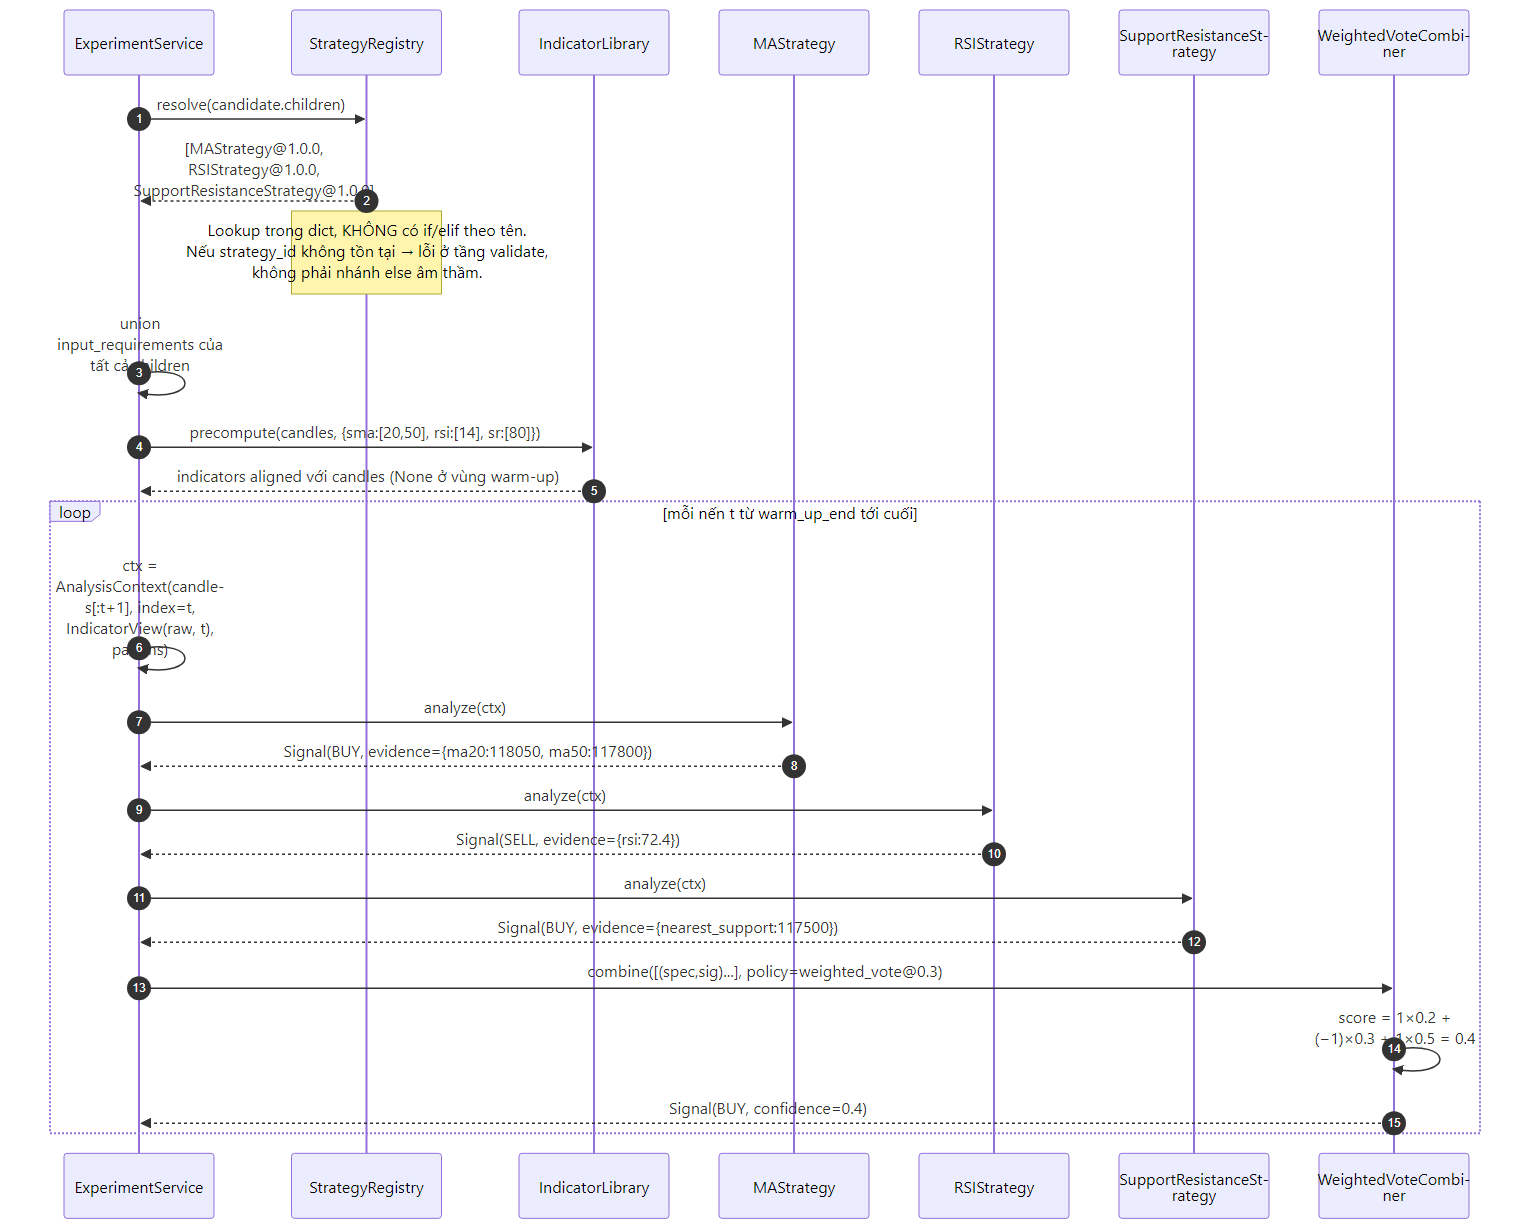
\includegraphics[width=\linewidth,height=0.75\textheight,keepaspectratio]{../blueprint/assets/diagrams-png/10-strategy-flow.png}
\end{column}
\end{columns}
\end{frame}

% Slide 21: Search Pipeline Flow
\begin{frame}{20. Runtime Flow: Pipeline Tìm Kiếm \& Chạy Backtest}
\begin{columns}[c]
\begin{column}{0.45\textwidth}
\begin{enumerate}
  \item \textbf{Atomic Transaction:} Ghi thí nghiệm và sự kiện Outbox cùng lúc.
  \item \textbf{Worker Lease Acquire:} Worker nhận việc qua Optimistic Lock \& gửi heartbeat.
  \item \textbf{Đa Phân Vùng:} Chạy tuần tự qua Train $\rightarrow$ Validation $\rightarrow$ Sealed Test.
  \item \textbf{Provenance:} Lưu Trade List, Sharpe, Drawdown \& cập nhật Leaderboard.
\end{enumerate}
\end{column}
\begin{column}{0.53\textwidth}
\centering
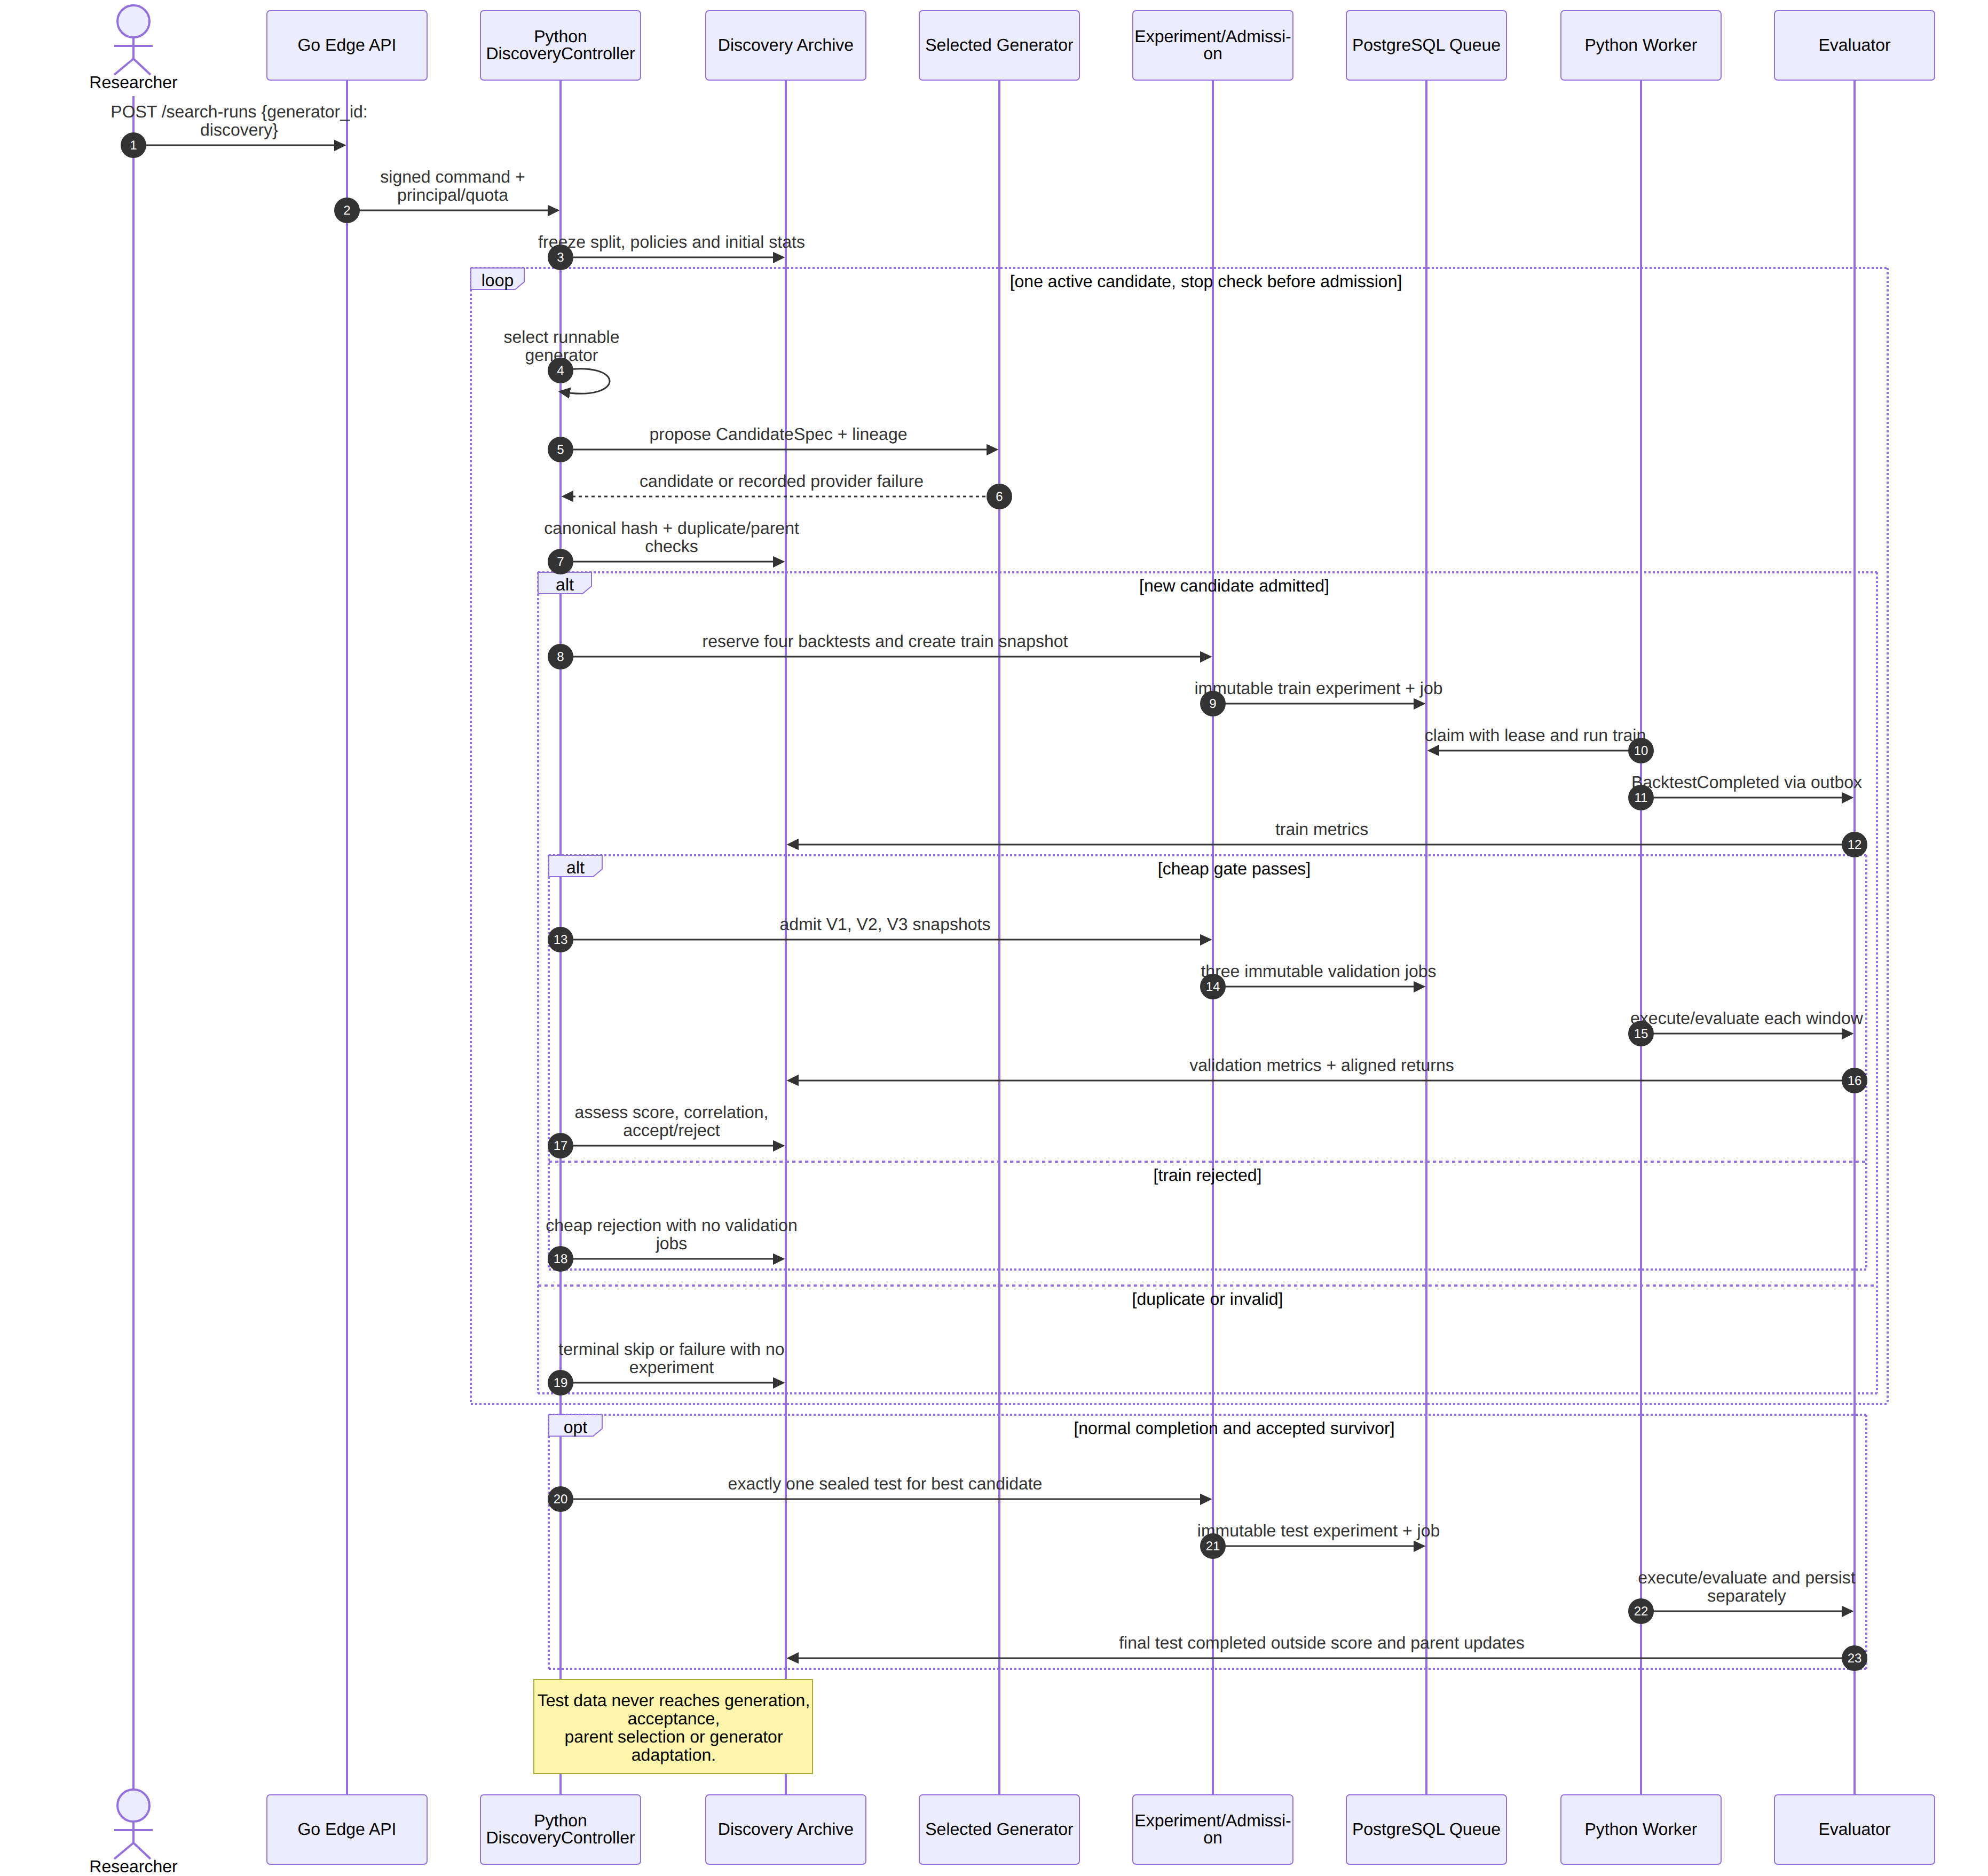
\includegraphics[width=\linewidth,height=0.75\textheight,keepaspectratio]{../blueprint/assets/diagrams-png/11-search-backtest-pipeline.png}
\end{column}
\end{columns}
\end{frame}

% Slide 22: News Pipeline Flow
\begin{frame}{21. Runtime Flow: Pipeline Crawl Tin Tức \& LLM Healing}
\begin{columns}[c]
\begin{column}{0.45\textwidth}
\begin{enumerate}
  \item \textbf{SSRF Check:} Duyệt nguồn từ \texttt{ApprovedSource}, thẩm tra DNS/IP.
  \item \textbf{Parser Extraction:} Trích xuất qua RSS/HTML parser chuẩn.
  \item \textbf{Quality Gate:} Bật \texttt{HtmlQualityGateFailed} nếu DOM thay đổi.
  \item \textbf{LLM Fallback:} Dùng LLM nhận diện nội dung chính xác.
  \item \textbf{Sentiment Score:} Chấm điểm [-1.0, 1.0] bất đồng bộ.
\end{enumerate}
\end{column}
\begin{column}{0.53\textwidth}
\centering
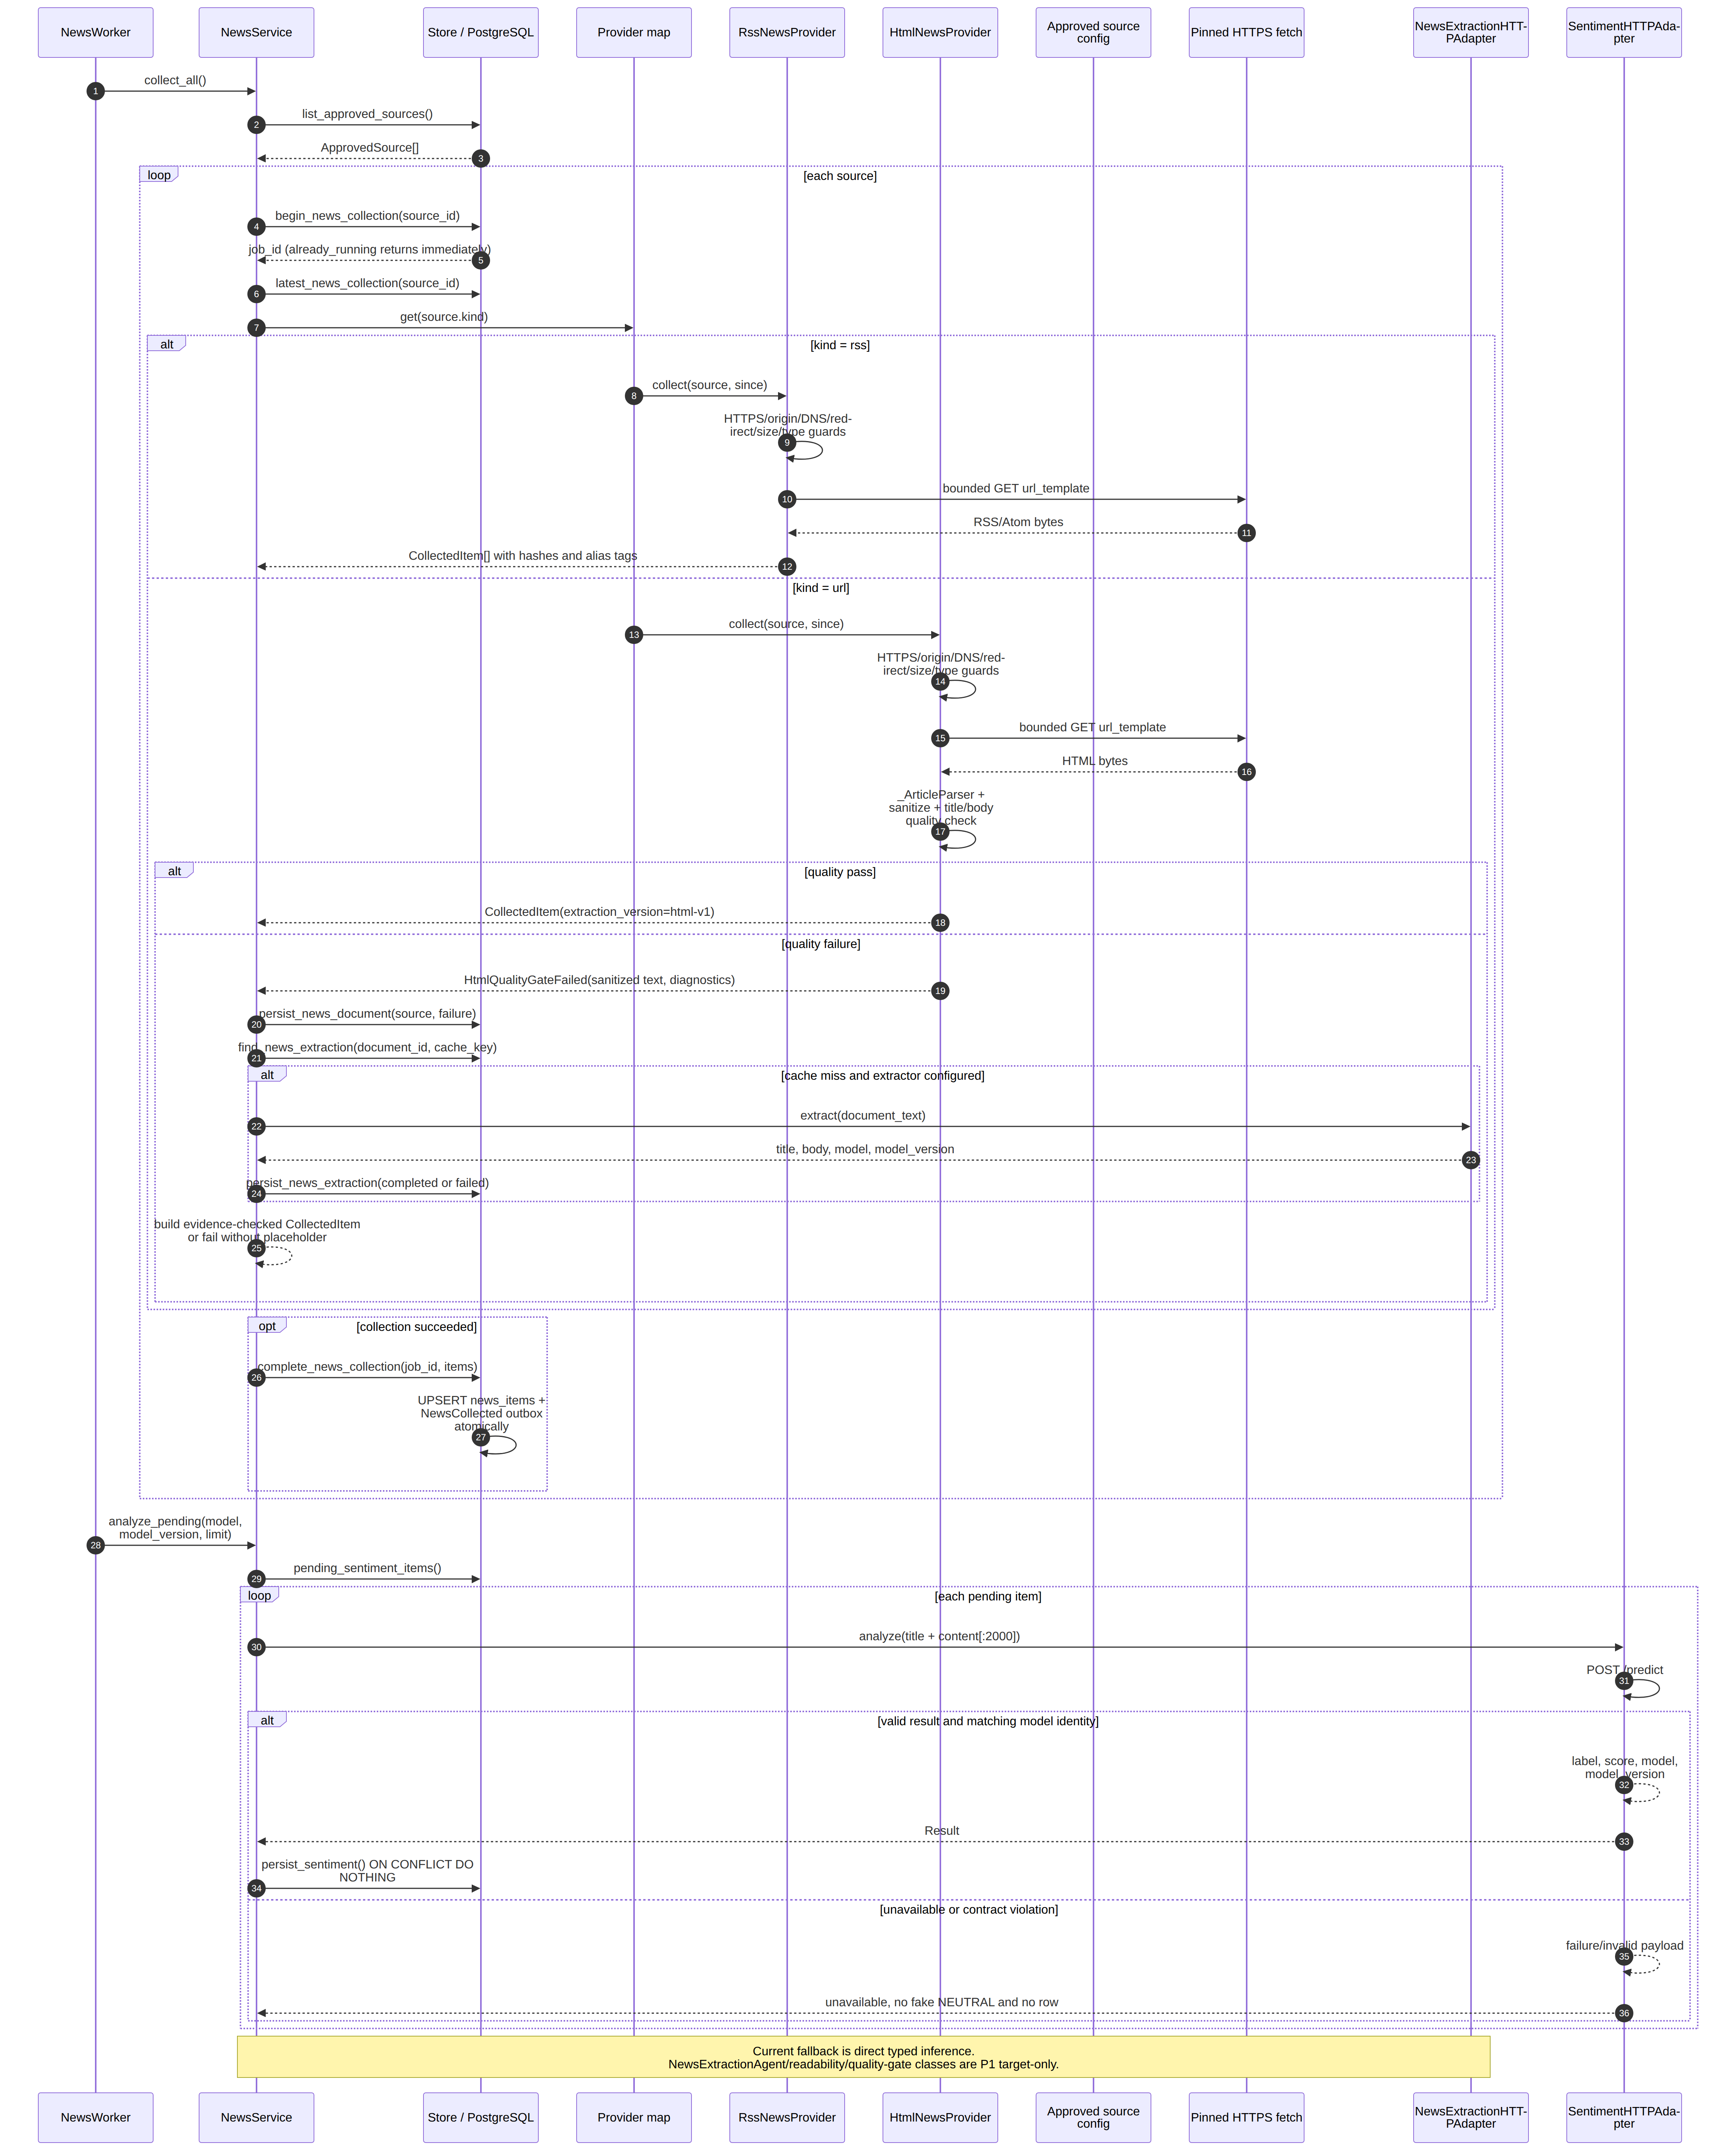
\includegraphics[width=\linewidth,height=0.75\textheight,keepaspectratio]{../blueprint/assets/diagrams-png/13-news-html-llm-pipeline.png}
\end{column}
\end{columns}
\end{frame}

% Slide 23: Defense in Depth
\begin{frame}{22. Kiến Trúc An Ninh: Phòng Thủ Đa Tầng}
\begin{columns}[c]
\begin{column}{0.45\textwidth}
\begin{itemize}
  \item \textbf{Authentication \& RBAC:} Xác thực JWT, cô lập dữ liệu người dùng.
  \item \textbf{Crawler SSRF Prevention:} Chặn private IP (127.0.0.1, 10.0.0.0/8, cloud metadata), chỉ duyệt HTTPS domain hợp lệ.
  \item \textbf{AST Sandbox:} Chặn lệnh nguy hiểm (\texttt{os.system}, \texttt{eval}, \texttt{subprocess}, socket) trong code AI.
  \item \textbf{Tool Boundary:} Giới hạn quyền gọi công cụ với DTO chặt chẽ.
\end{itemize}
\end{column}
\begin{column}{0.53\textwidth}
\centering
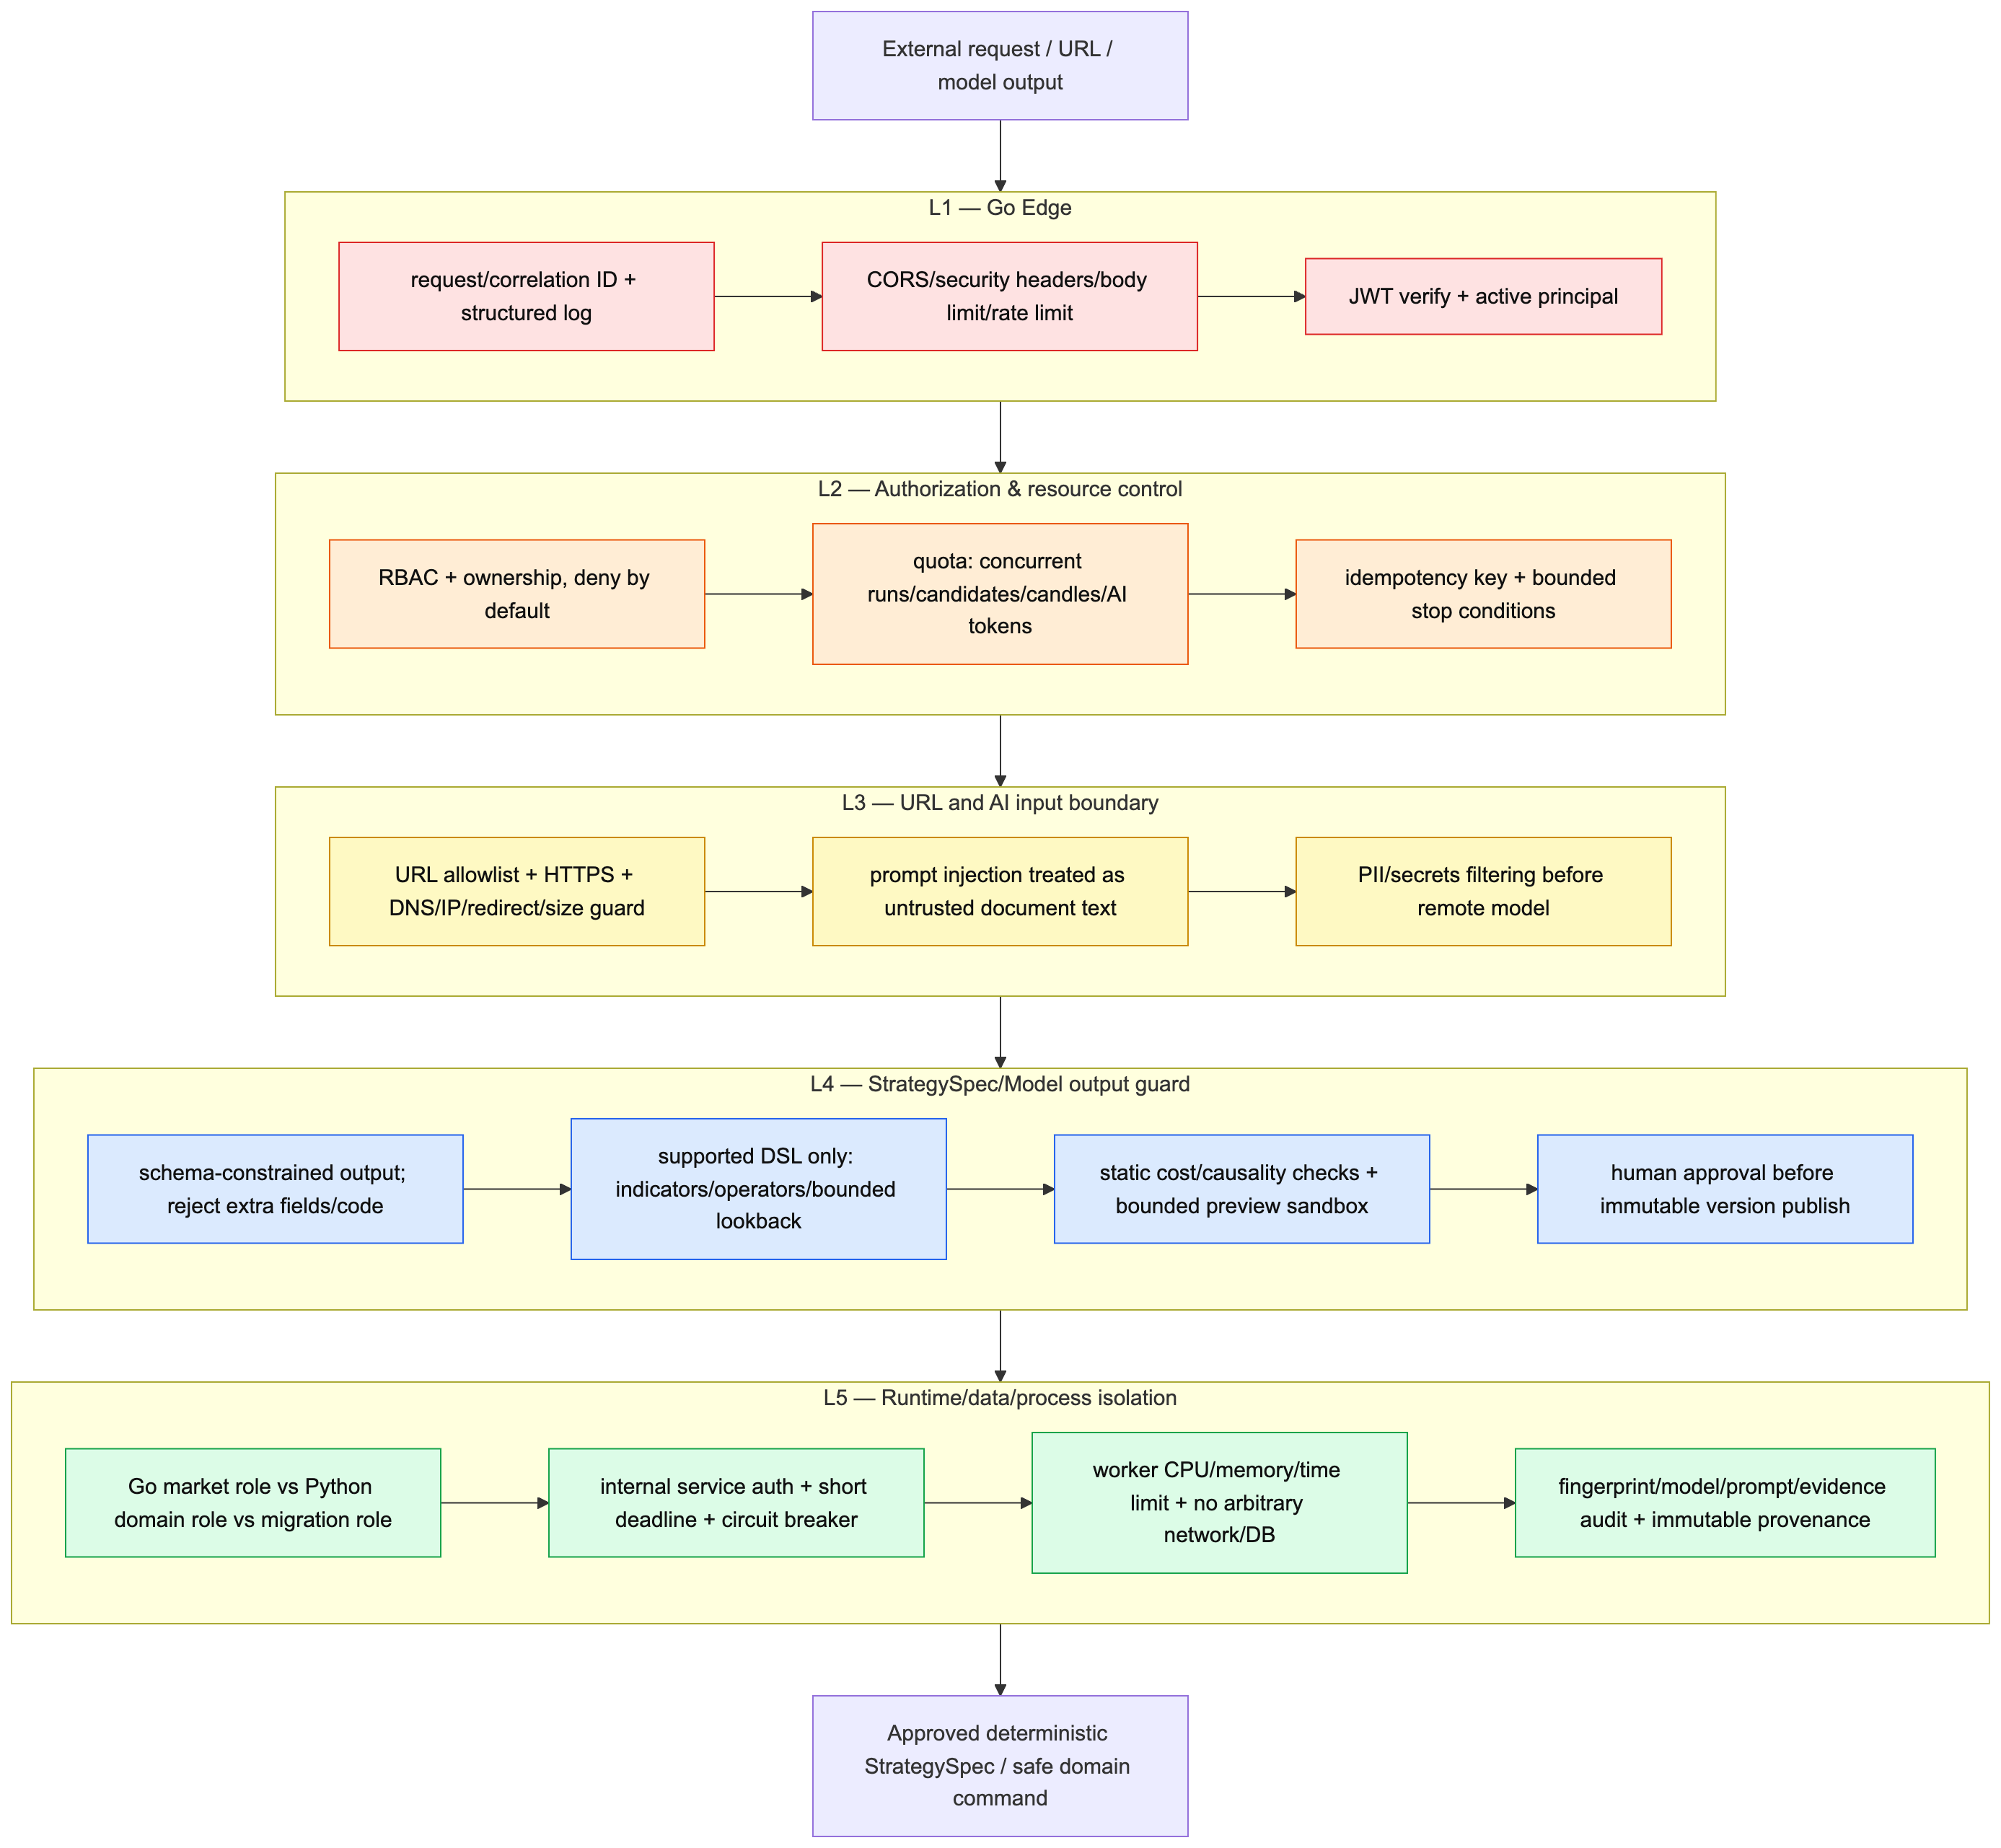
\includegraphics[width=\linewidth,height=0.75\textheight,keepaspectratio]{../blueprint/assets/diagrams-png/14-defense-in-depth.png}
\end{column}
\end{columns}
\end{frame}

% Slide 24: Scalability
\begin{frame}{23. Khả Năng Mở Rộng (Scalability) \& Benchmark}
\begin{columns}[c]
\begin{column}{0.45\textwidth}
\begin{itemize}
  \item \textbf{Stateless Scale-Out:}
  \begin{itemize}
    \item Nhân bản Python Worker pool theo tải CPU.
    \item Hàng đợi Postgres Outbox có chỉ mục B-Tree \& phân đoạn.
  \end{itemize}
  \item \textbf{Kịch bản Benchmark:}
  \begin{itemize}
    \item Tốc độ xử lý $> 1,500$ backtests/phút trên 4 workers.
    \item Độ trễ API nến \& leaderboard $\le 120$ms ($p95$).
    \item Sẵn sàng chịu tải $100,000$ backtests.
  \end{itemize}
\end{itemize}
\end{column}
\begin{column}{0.53\textwidth}
\centering
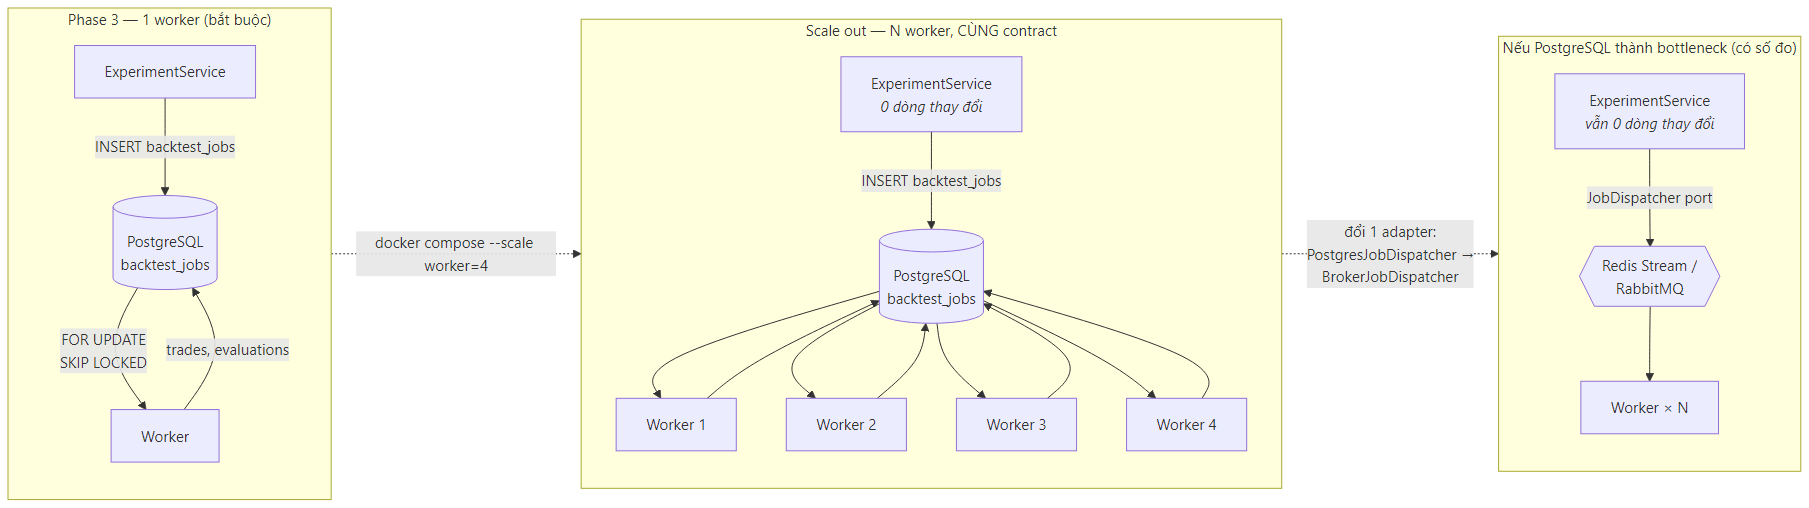
\includegraphics[width=\linewidth,height=0.75\textheight,keepaspectratio]{../blueprint/assets/diagrams-png/15-job-queue-scale.png}
\end{column}
\end{columns}
\end{frame}

% Slide 25: Fault Tolerance
\begin{frame}{24. Xử Lý Sự Cố \& Khôi Phục Tự Động}
\begin{columns}[c]
\begin{column}{0.45\textwidth}
\begin{itemize}
  \item \textbf{Worker Lease Takeover:} Heartbeat 10s. Nếu worker crash, sau 30s hết hạn lease worker khác sẽ tiếp quản job.
  \item \textbf{Tính Idempotent:} Dùng \texttt{idempotency\_key} và unique constraint trên CSDL, không bao giờ chạy trùng kết quả.
  \item \textbf{Cô lập lỗi tuyệt đối:} 1 chiến lược lỗi chỉ fail job đó, không sập worker hay gateway.
\end{itemize}
\end{column}
\begin{column}{0.53\textwidth}
\centering
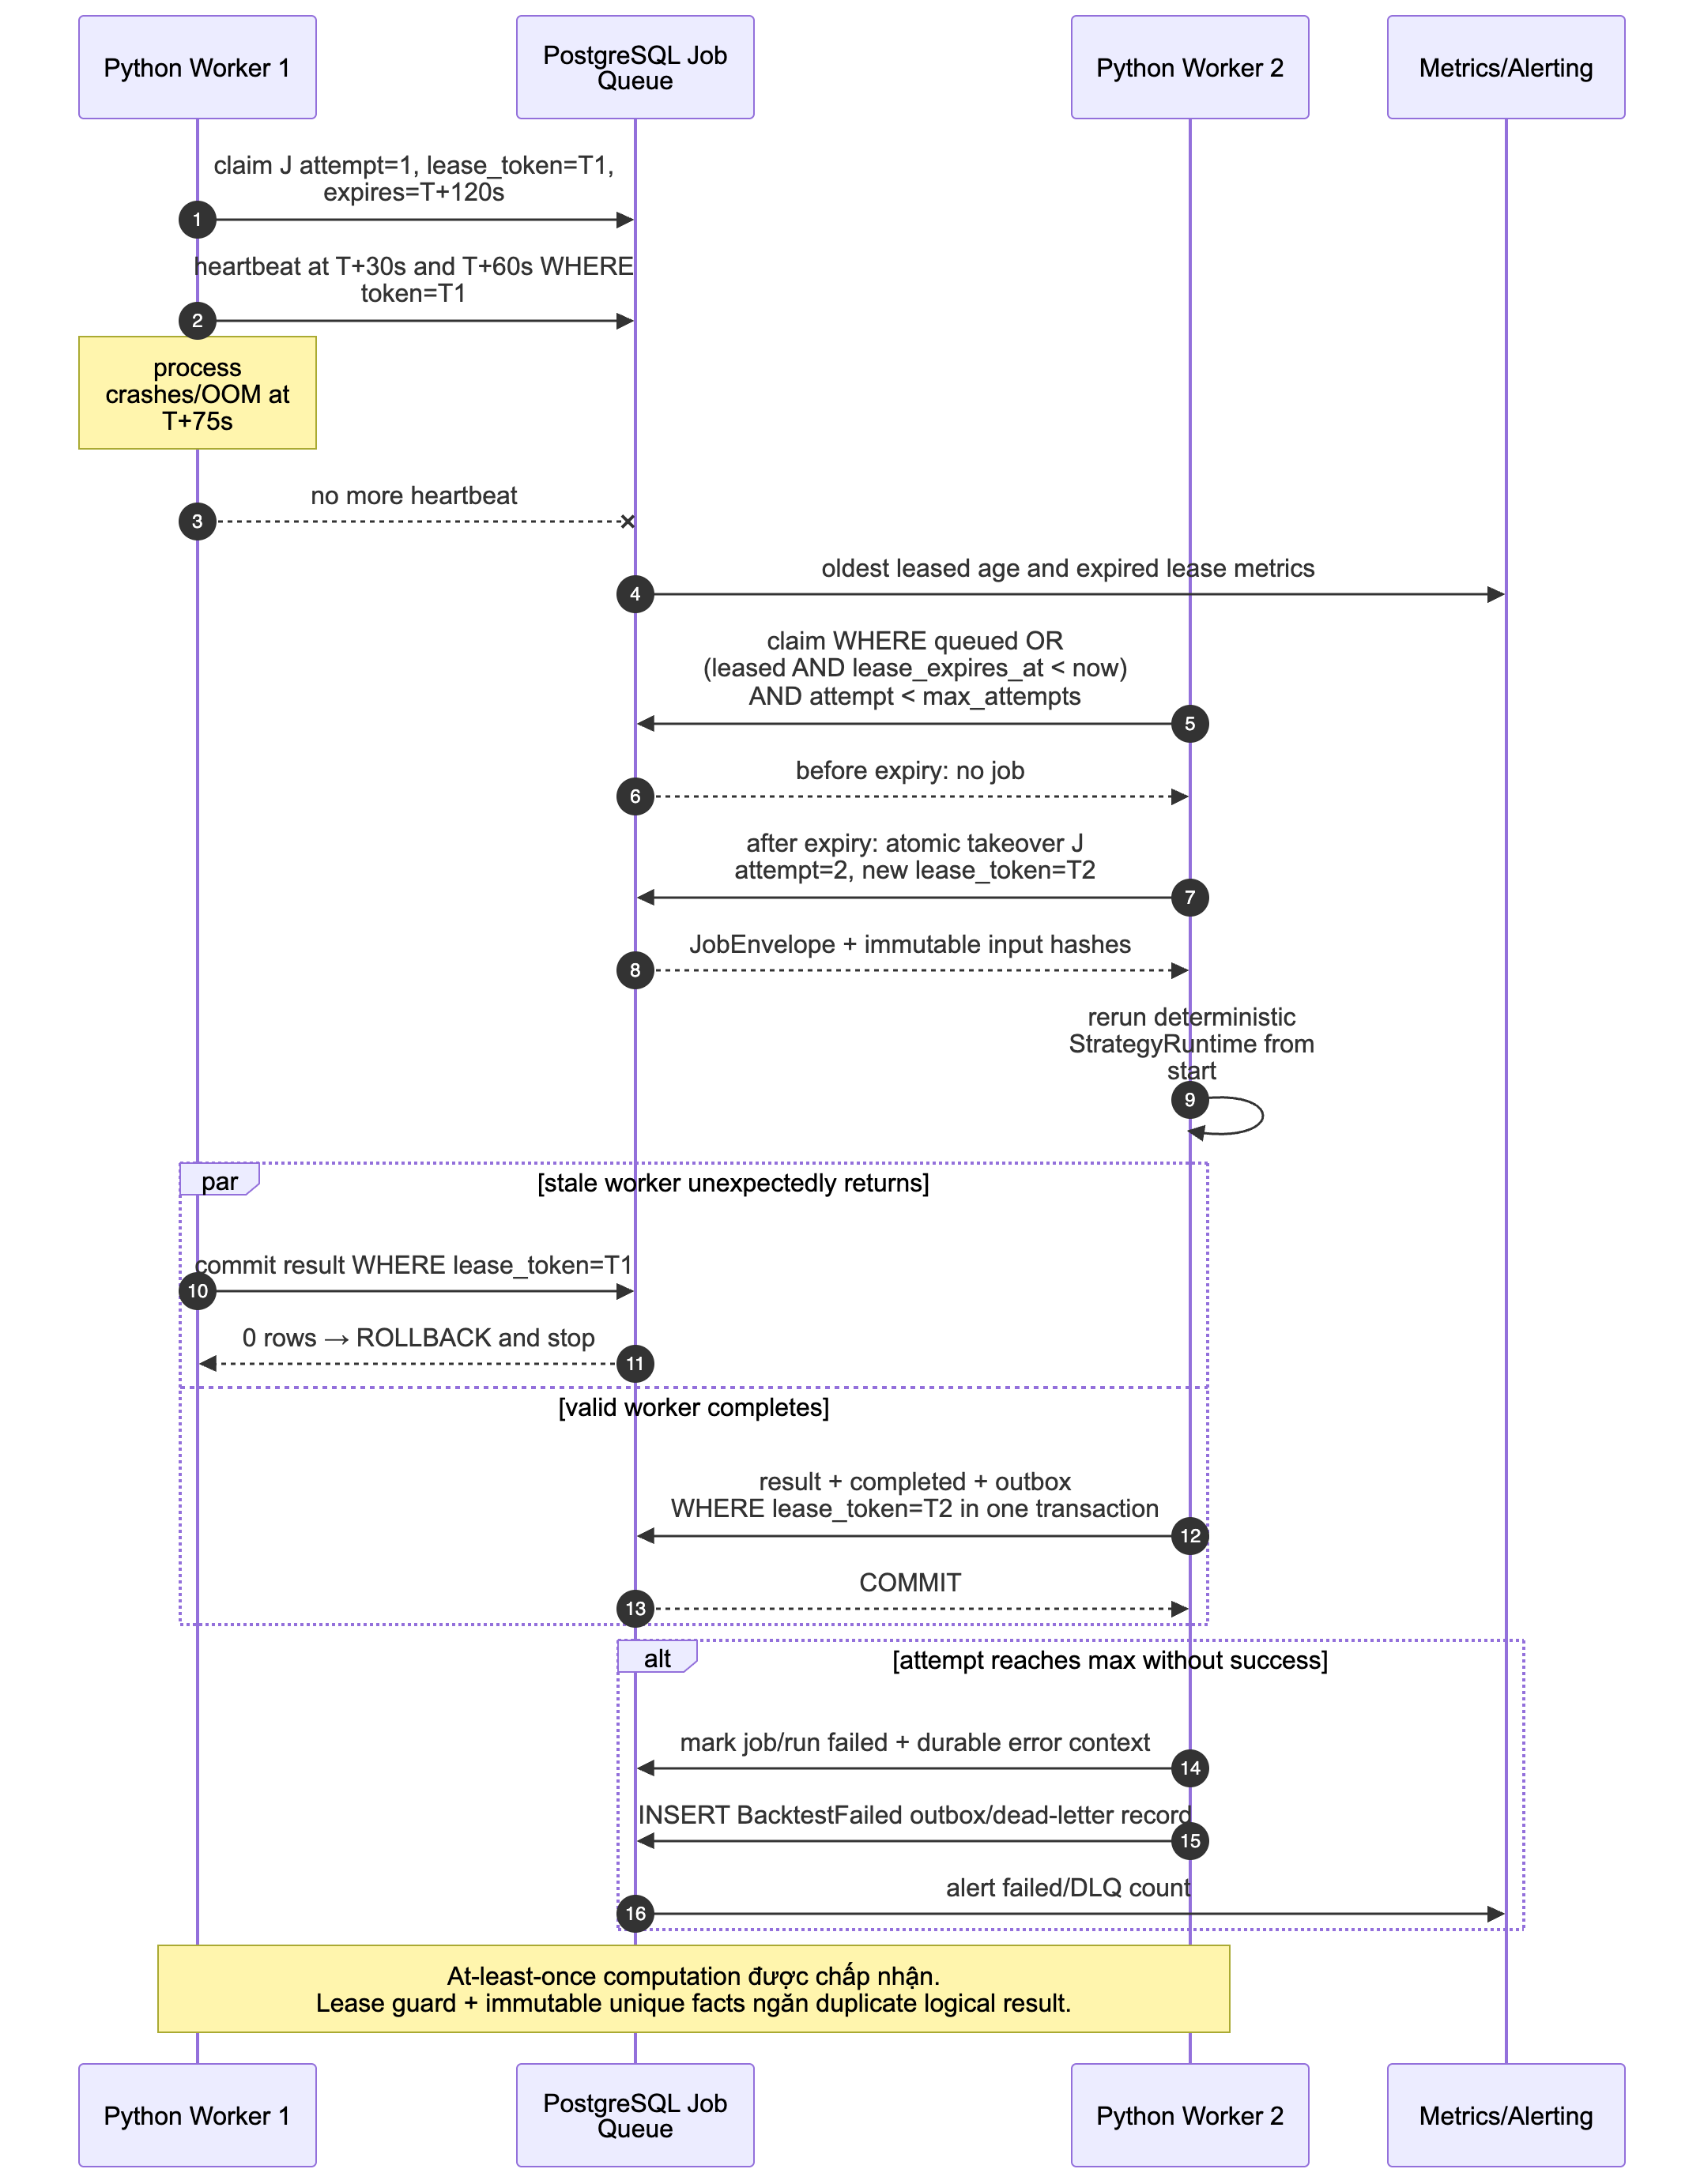
\includegraphics[width=\linewidth,height=0.75\textheight,keepaspectratio]{../blueprint/assets/diagrams-png/18-worker-lease-takeover.png}
\end{column}
\end{columns}
\end{frame}

% Slide 26: Deployment Topology
\begin{frame}{25. Triển Khai Thực Tế \& MLOps}
\begin{columns}[c]
\begin{column}{0.45\textwidth}
\begin{itemize}
  \item \textbf{Docker Compose Topology:} Next.js Web, Go Edge, Python Research, Background Workers, AI Service, PostgreSQL.
  \item \textbf{Healthchecks:} Endpoint \texttt{/healthz} \& \texttt{/readyz} tự động restart container khi deadlock.
  \item \textbf{MLOps Configuration:} System prompt và LLM API keys đặt trong \texttt{.env}, không hardcode.
\end{itemize}
\end{column}
\begin{column}{0.53\textwidth}
\centering
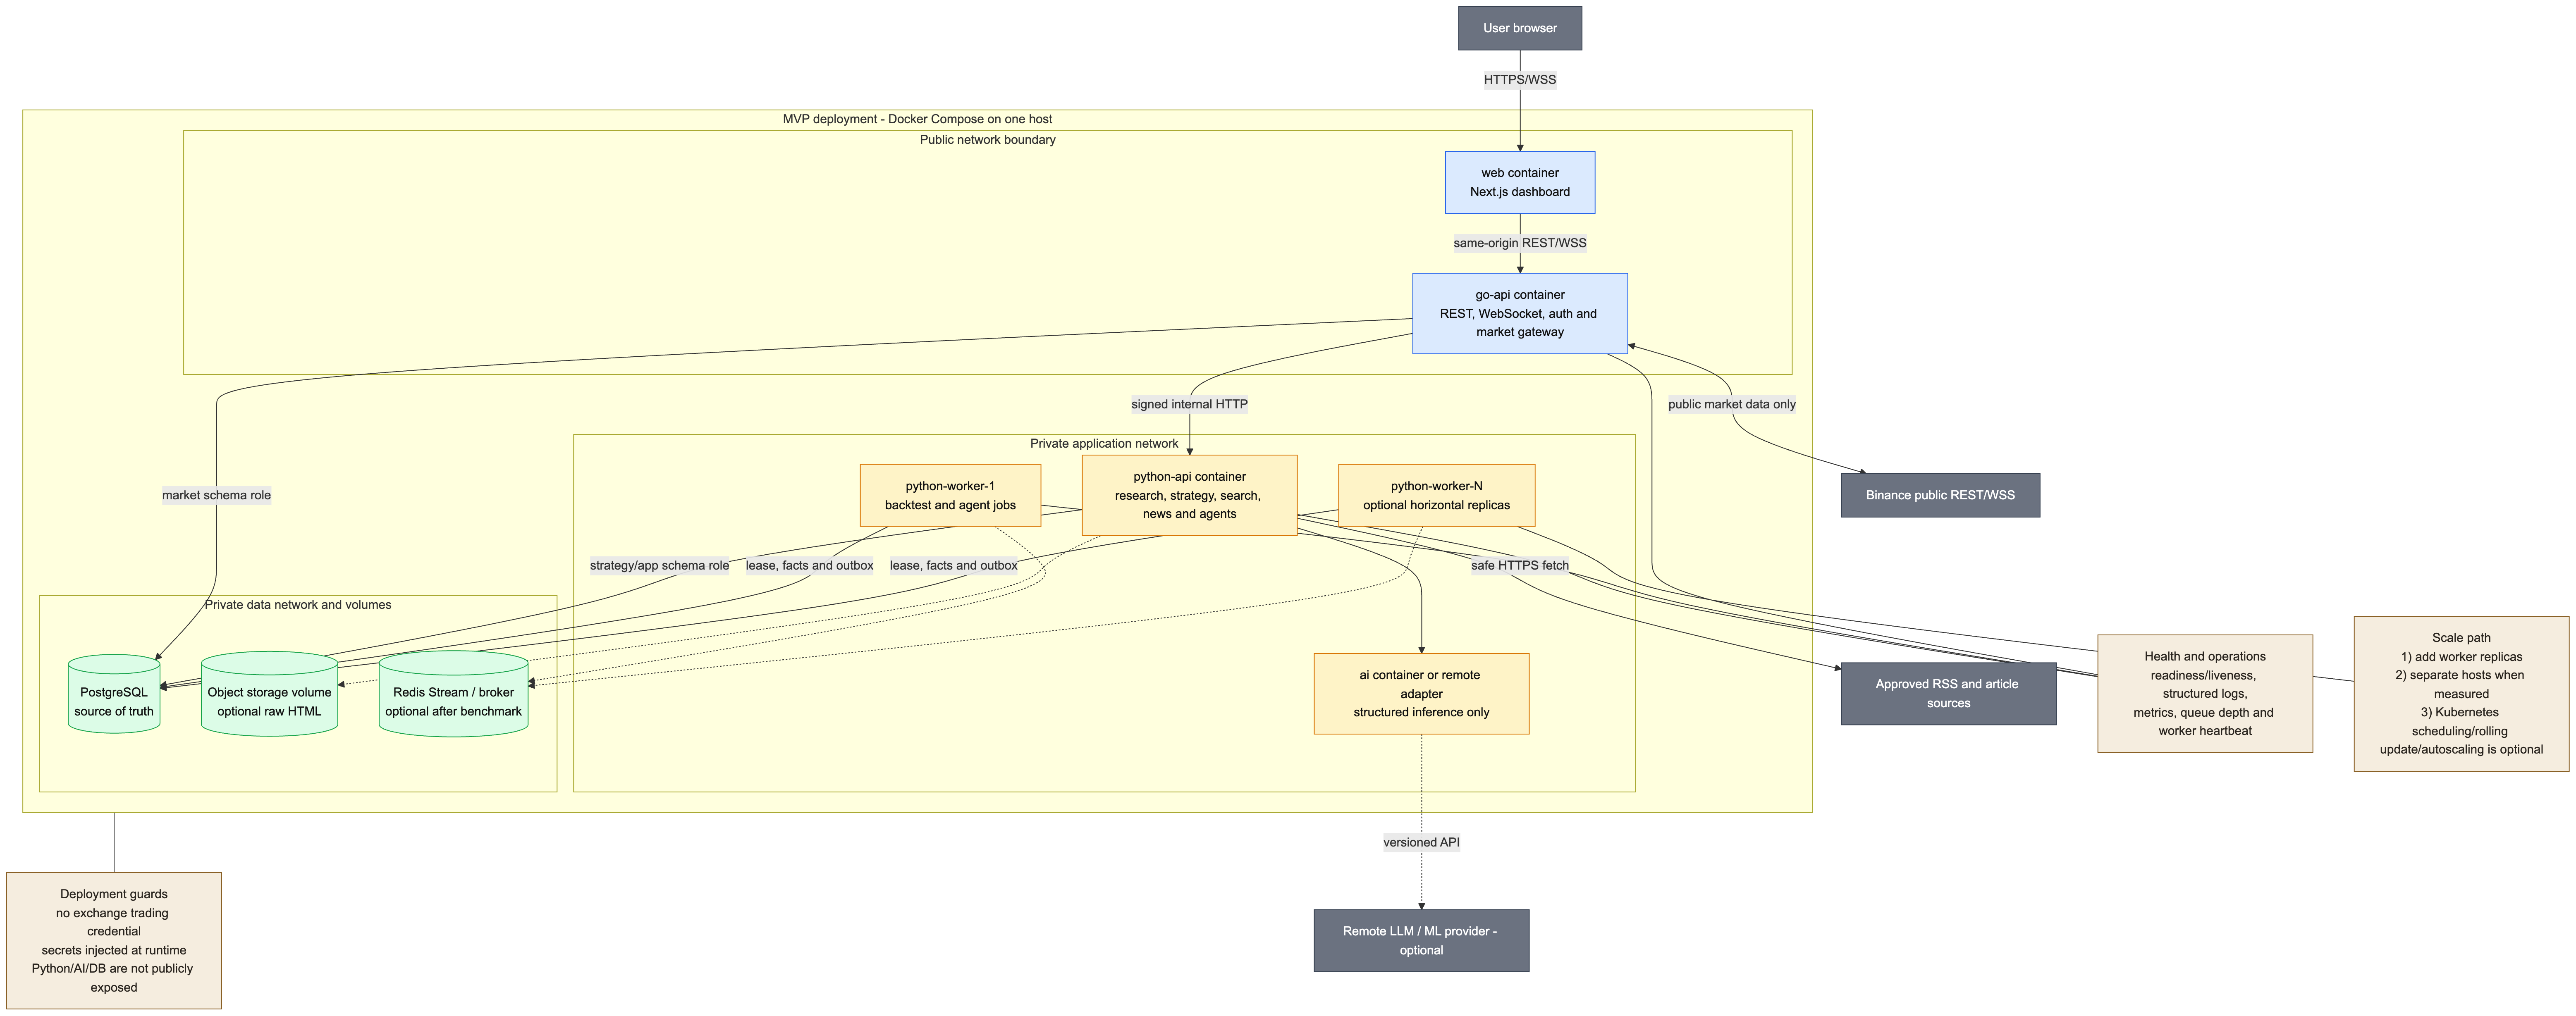
\includegraphics[width=\linewidth,height=0.75\textheight,keepaspectratio]{../blueprint/assets/diagrams-png/39-deployment-topology.png}
\end{column}
\end{columns}
\end{frame}

% Slide 27: Tradeoffs Matrix
\begin{frame}{26. Ma Trận Đánh Giá Đánh Đổi Kiến Trúc}
\resizebox{\textwidth}{!}{%
\begin{tabular}{lp{3.2cm}p{3cm}p{6cm}}
\toprule
\textbf{Lựa Chọn} & \textbf{Phương Án Chọn} & \textbf{Phương Án Khác} & \textbf{Lý Do \& Đánh Đổi (Rationale)} \\
\midrule
\textbf{Tổng thể} & \textbf{Modular Monolith} & Microservices & Giảm độ phức tạp vận hành mạng, ranh giới rõ qua contracts. \\
\textbf{Lưu trữ} & \textbf{Postgres + B-Tree} & ClickHouse / InfluxDB & Giữ ACID cho Outbox \& Thí nghiệm; B-Tree đủ tải hàng triệu nến. \\
\textbf{Hàng đợi} & \textbf{Postgres Outbox} & Kafka / RabbitMQ / Redis & Loại bỏ Dual-write, đảm bảo ACID nguyên tử không cần broker ngoài. \\
\textbf{Mã AI sinh} & \textbf{AST + Sandbox} & Docker-in-Docker & Khởi tạo tức thì ($<10$ms), kiểm soát an toàn không tốn container. \\
\textbf{Sentiment} & \textbf{Hybrid Rule+LLM} & Pure Realtime LLM & Tiết kiệm token API, tránh nghẽn luồng crawl tin. \\
\bottomrule
\end{tabular}}
\end{frame}

% Slide 28: Replaceability
\begin{frame}{27. Khả Năng Thay Thế \& Mở Rộng Tương Lai}
\begin{columns}[c]
\begin{column}{0.45\textwidth}
\begin{itemize}
  \item \textbf{Thay thế Market Provider:} \texttt{MarketProviderAdapter} cho phép đổi sang OKX, Bybit, Coinbase mà không sửa Frontend hay Engine.
  \item \textbf{Mở rộng Search Algorithm:} Tích hợp Reinforcement Learning (PPO) qua \texttt{ISearchAlgorithm}.
  \item \textbf{Mở rộng News Sources:} Bổ sung CryptoPanic, CoinDesk API qua cấu hình nguồn.
\end{itemize}
\end{column}
\begin{column}{0.53\textwidth}
\centering
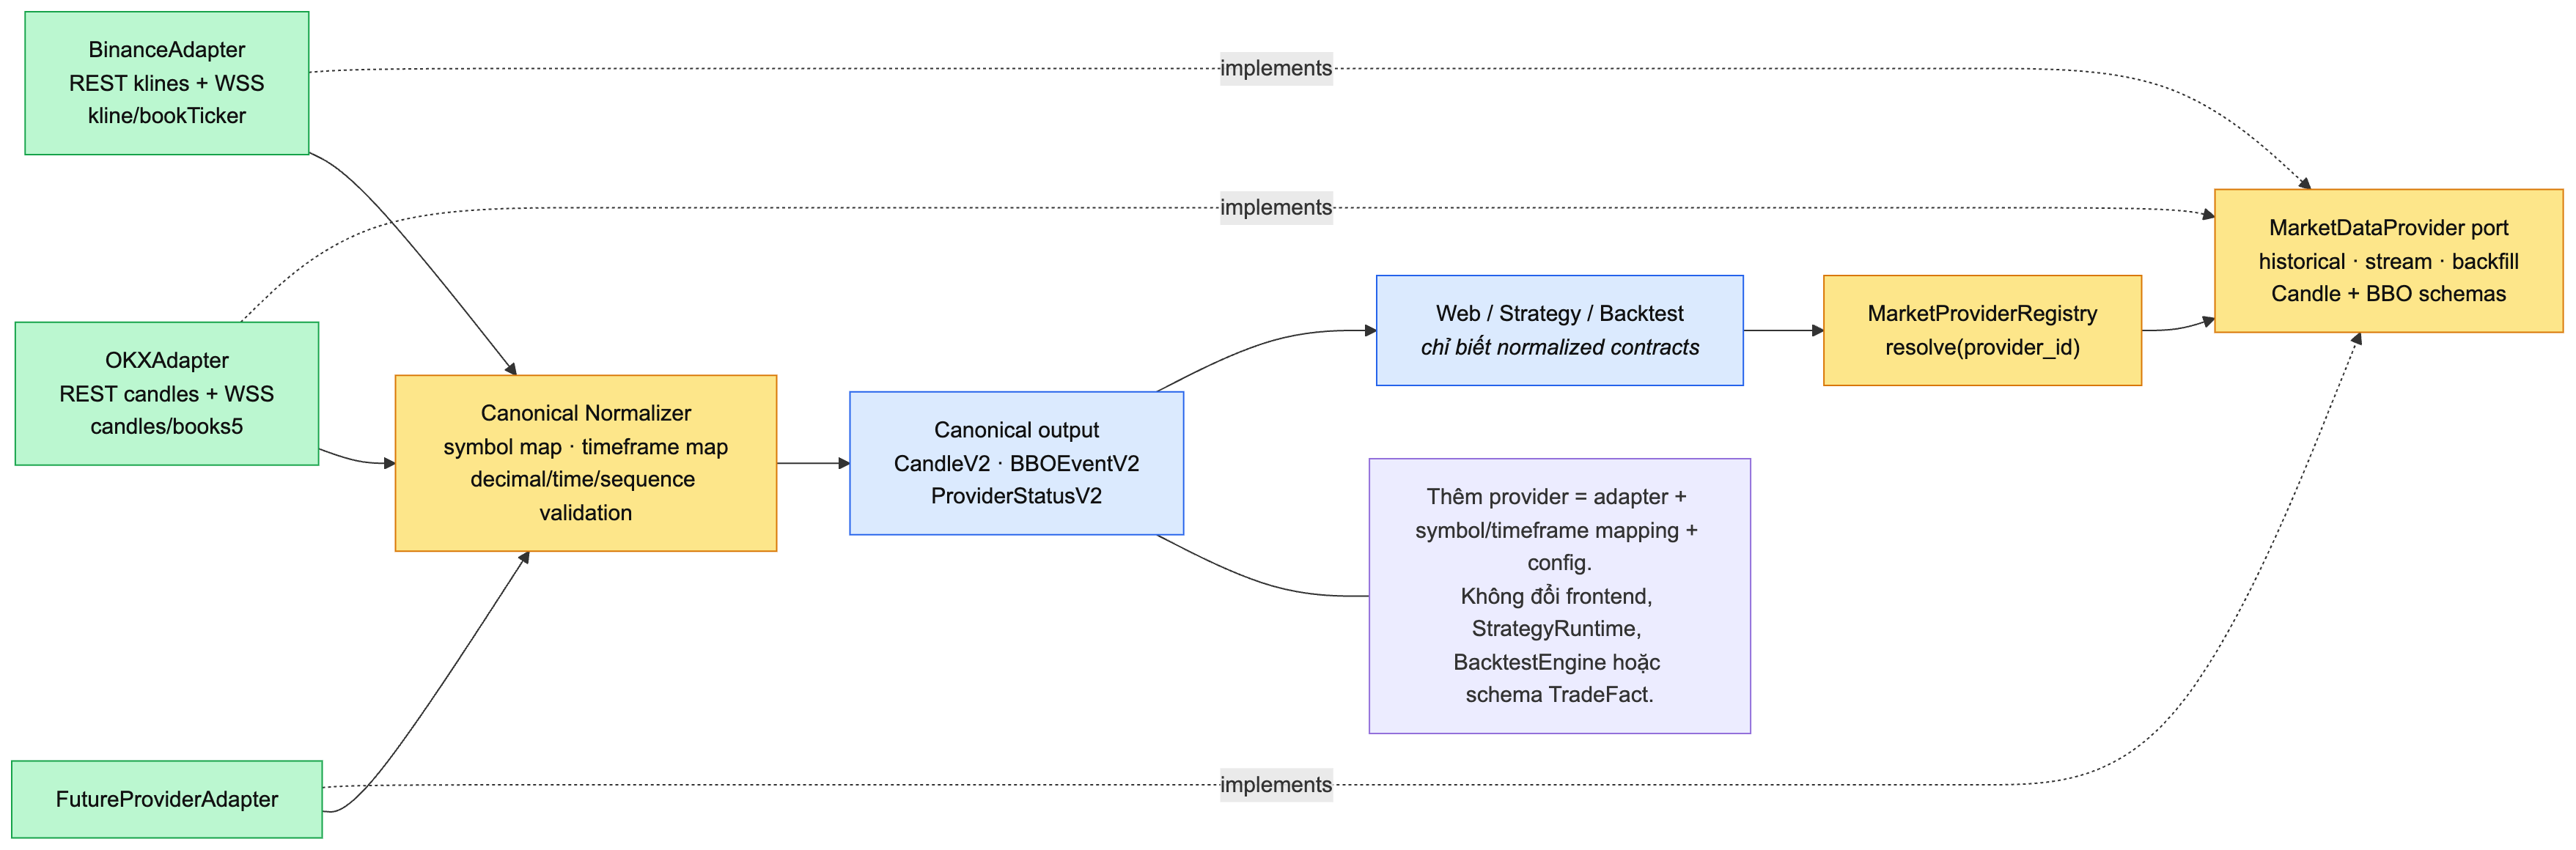
\includegraphics[width=\linewidth,height=0.75\textheight,keepaspectratio]{../blueprint/assets/diagrams-png/20-market-provider-replaceability.png}
\end{column}
\end{columns}
\end{frame}

% Slide 29: Summary & QA
\begin{frame}{28. Tổng Kết Đồ Án \& Giá Trị Kiến Trúc}
\begin{columns}[T]
\begin{column}{0.48\textwidth}
\begin{block}{\textbf{[Thành Quả Đạt Được]}}
\begin{itemize}
  \item $\checkmark$ \textbf{Chuỗi Quyết Định Rõ Ràng:} Bám sát ASRs \& Quality Attributes.
  \item $\checkmark$ \textbf{Chống God Service:} 5 subsystem rành mạch.
  \item $\checkmark$ \textbf{Multi-Agent \& Self-Repair:} Tự sửa code \& chống Overfitting.
  \item $\checkmark$ \textbf{Chịu Tải \& Phục Hồi:} Hàng đợi phân tán \& Lease Takeover.
\end{itemize}
\end{block}
\vspace{0.5em}
\centering
\textbf{[PHẦN HỎI - ĐÁP (Q \& A)]} \\
\textit{Cảm ơn Thầy và các bạn đã lắng nghe!}
\end{column}
\begin{column}{0.48\textwidth}
\begin{block}{\textbf{[Minh Chứng Đầy Đủ]}}
\begin{itemize}
  \item \textbf{39 Sơ Đồ Blueprint \& Specs:} C4 (L1-L3), UML Class, State Machine, Topology.
  \item \textbf{5 Màn Hình Sẵn Sàng:}
  \begin{enumerate}
    \item Realtime Market Chart \& Indicators
    \item Strategy Authoring \& Registry
    \item Async Backtest \& Trade Visualization
    \item Search Loop \& Leaderboard
    \item News Crawler \& Sentiment
  \end{enumerate}
  \item \textbf{Test Tự Động \& Benchmark Đầy Đủ.}
\end{itemize}
\end{block}
\end{column}
\end{columns}
\end{frame}

\end{document}
